\documentclass[12pt,twoside]{article}

\usepackage[T1]{fontenc}
\usepackage[utf8]{inputenc}
\usepackage[spanish]{babel}
\usepackage{hyperref}


\let\layoutspanish\relax
\addto\captionsspanish{\def\tablename{Tabla}} % para que escriba "Tabla" en lugar de "Cuadro"
\unaccentedoperators  % para que no acentúe los operadores

% Área de impresión de una página:
\usepackage[a4paper]{geometry}
  \geometry{hmargin={2.5cm,2.5cm},height=22cm}

% Formato de algunas distancias:
\renewcommand{\baselinestretch}{1.2}    % separación entre líneas de un mismo párrafo
\setlength{\partopsep}{0pt}
\setlength{\itemsep}{0pt}
\setlength{\topsep}{0pt}
\setlength{\parsep}{0pt}
\setlength{\parskip}{0.25\baselineskip}   % separación entre párrafos

\renewcommand{\textfraction}{0.1}   % mínima fracción de la página para el texto
\renewcommand{\topfraction}{1}      % máxima fracción de la página para objetos flotantes en la parte superior
\renewcommand{\bottomfraction}{1}
\renewcommand{\floatpagefraction}{1}

\setcounter{totalnumber}{5}
\setcounter{topnumber}{3}
\setcounter{bottomnumber}{2}

% Adaptación de las "caption" de los entorns "figure" y "table":
\usepackage{caption}
\captionsetup{
  labelfont={up,bf},%
  font={small,sl},%
}

% Indentación del primer párrafo de una sección:
\usepackage{indentfirst}

% Definición del color grisclaro en la salida PDF:
\usepackage[pdftex]{color}

% Gráficos:
\usepackage[pdftex]{graphicx}

% Paquetes recomendados para la inclusión de fórmulas matemáticas:
\usepackage{amsmath}
\allowdisplaybreaks  % para que pueda partir fórmulas que ocupan más de una línea, necesita el paquete anterior
\usepackage{amssymb} % para cargar algunos símbolos como \blacksquare y \square
\usepackage{amsfonts} % para cargar algunas fuentes en estilo matemático
\usepackage{enumerate}
% Teoremas (se pueden definir todos los que se necesiten):

\newtheorem{theorem}{Teorema}[section]
\newtheorem{proposition}[theorem]{Proposición}
\newtheorem{definition}[theorem]{Definición}
\newtheorem{lemma}[theorem]{Lema}
\newtheorem{corollary}[theorem]{Corolario}
\newtheorem{example}[theorem]{Ejemplo}
\newtheorem{app}[theorem]{Aplicación}
\newtheorem{remark}[theorem]{Observación}
\newtheorem{agrad}[theorem]{Agradecimiento}
\newtheorem{algo}[theorem]{Algoritmo}
\newtheorem{axiom}[theorem]{Axioma}
\newtheorem{case}[theorem]{Caso}
\newtheorem{conclu}[theorem]{Conclusión}
\newtheorem{conjectura}[theorem]{Conjetura}
\newtheorem{notac}[theorem]{Notación}
\newtheorem{soluc}[theorem]{Solución}
\newtheorem{summary}[theorem]{Sumario}


\newtheorem{proof}[theorem]{Demostración.}
\renewenvironment{proof}{\emph{Demostración.}} {\quad \hfill $\blacksquare$ \newline} % para que aparezca un cuadrado negro al acabar la demostración


% Definición de cabeceras y pies de página:

\usepackage{fancyhdr}                     % para definir distintos tipos de cabeceras y pies de página

\newcommand{\RunningAuthor}{Marina Peñalver Ripoll}
\newcommand{\Author}[1]{\renewcommand{\RunningAuthor}{#1}}
\renewcommand{\leftmark}{\RunningAuthor}

\newcommand{\RunningTitle}{Trabajo de fin de grado}
\newcommand{\Title}[1]{\renewcommand{\RunningTitle}{#1}}
\renewcommand{\rightmark}{\RunningTitle}

\pagestyle{fancy}
\fancyhf{}
\fancyhead[LO]{\small \slshape \leftmark}    % lo que aparece en la parte izquierda de la páginas impares
\fancyhead[RE]{\small \slshape \rightmark}   % lo que aparece en la parte derecha de las páginas pares
\fancyhead[RO,LE]{\small \slshape \thepage}  % el número de página aparece en la parte exterior de la cabecera

\renewcommand{\headrulewidth}{0.6pt}         % grueso de la línea horizontal por debajo de la cabecera de la página
\renewcommand{\footrulewidth}{0pt}           % grueso de la línea horizontal por encima del pie de página
                                             % en este caso está vacío
\setlength{\headheight}{1.5\headheight}      % aumenta la altura de la cabecera en una parte y media

\fancypagestyle{plain}{%                     % redefinición del estilo de página 'plain'
  \fancyhf{}                                 % limpia todas las cabeceras y pies de página
  \setlength{\headwidth}{\textwidth}
  \fancyfoot[C]{\small \slshape \thepage}    % excepto el centro del pie de página
  \renewcommand{\headrulewidth}{0pt}
  \renewcommand{\footrulewidth}{0pt}
  }

% Instrucciones que se usan frecuentemente
\newcommand{\abs}[1]{\ensuremath{|#1|}}
\newcommand{\ar}{\text{AR}}
\newcommand{\ma}{\text{MA}}
\newcommand{\arma}{\text{ARMA}}
\newcommand{\arima}{\text{ARIMA}}
\newcommand{\wn}{\text{WN}(0, \sigma^2)}

% Datos del trabajo y autor:
\title{Métodos no clásicos de series temporales en data science}
\author{Marina Peñalver Ripoll\\*[1em]
\begin{minipage}{0.75\textwidth}
\footnotesize \itshape
\begin{center}
Universidad de Alicante \\
4º de Grado en Matemáticas
\end{center}
\end{minipage}
}
\date{Julio 2021}

% Para incluir paginas de otro pdf (por ejemplo, la de la portada):
\usepackage{pdfpages}

\begin{document}
%-------------------------------------------------------------------------------------------------------


% PORTADA
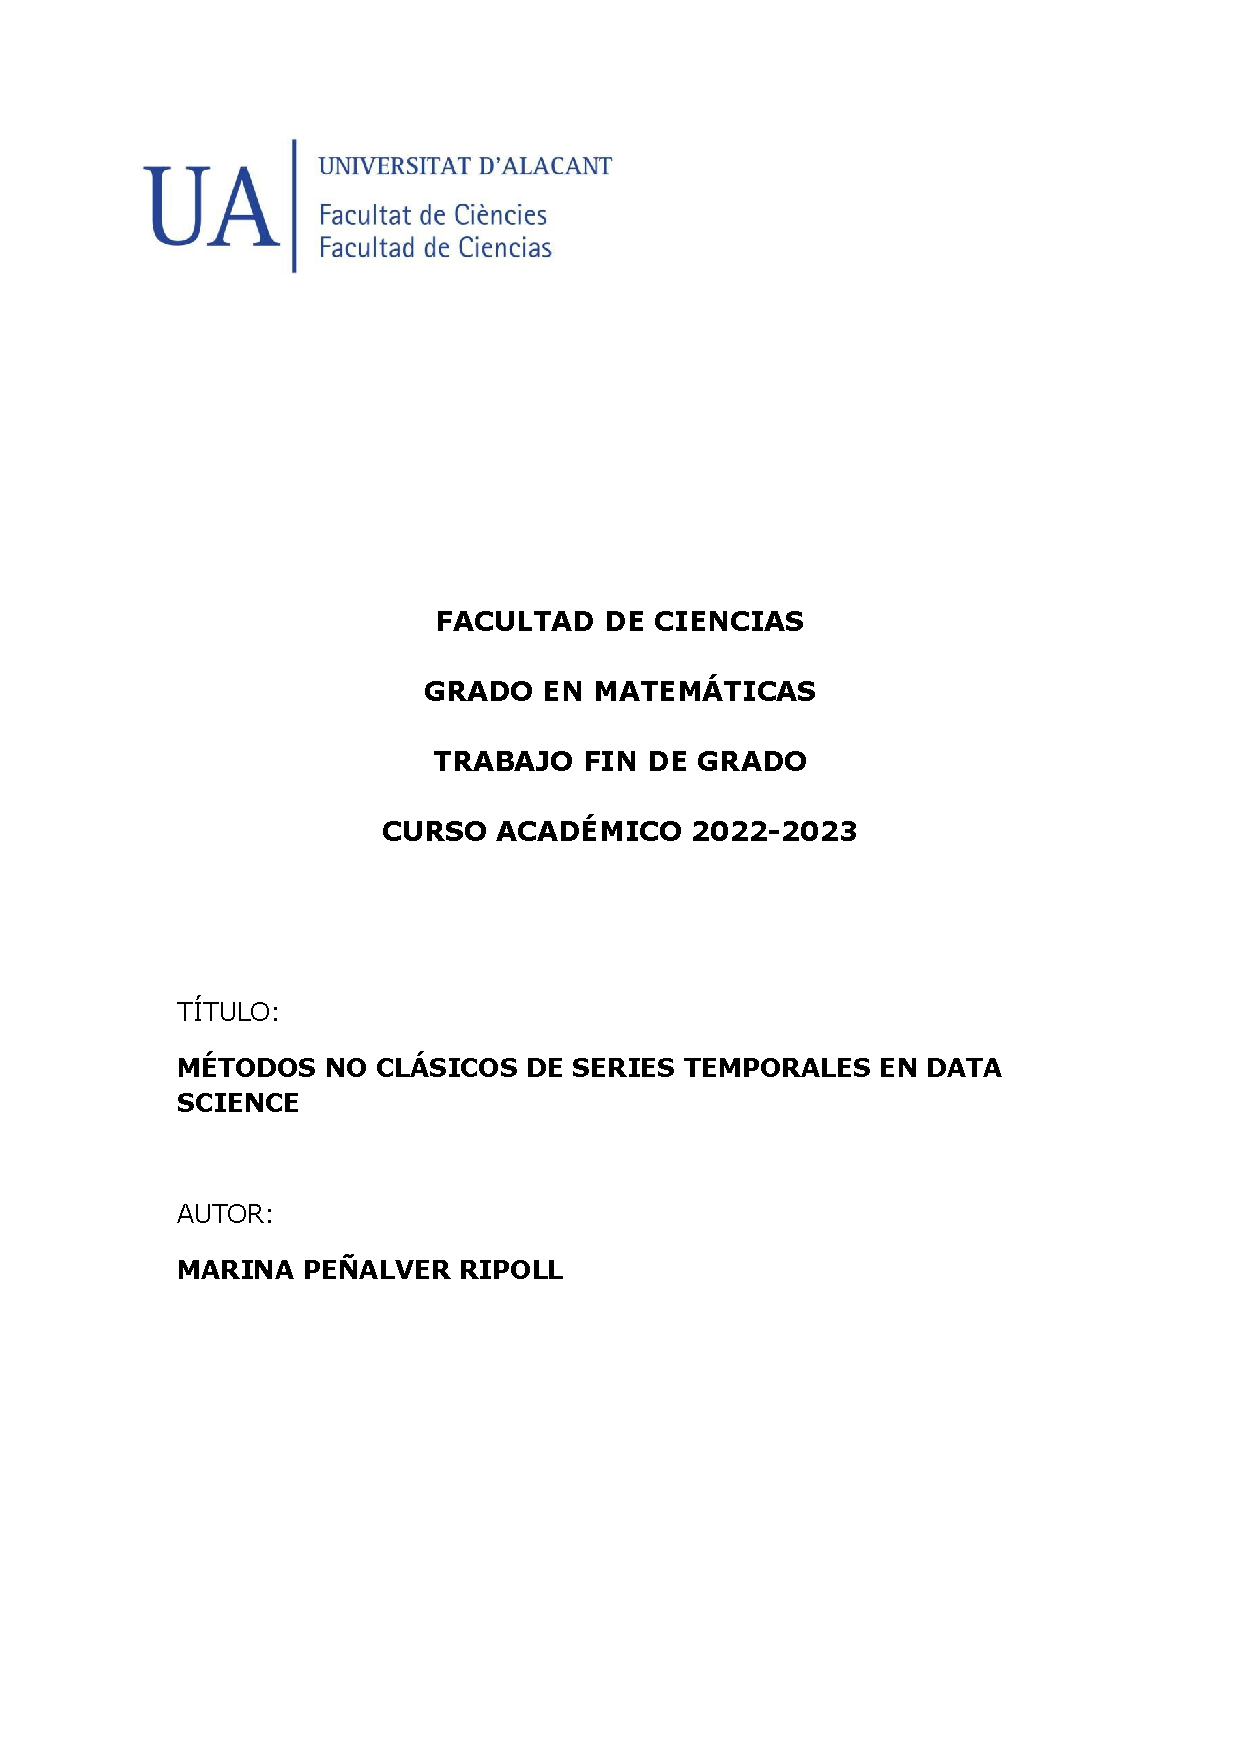
\includepdf[pages=1]{imagenes/anexo-1-portada-memoria-tfg-matematicas.pdf}

%-------------------------------------------------------------------------------------------------------





% RESUMEN
\section*{Resumen}
Las series temporales son un conjunto de datos ordenados que comparten un factor temporal. El aumento en los datos disponibles ha provocado un aumento en la demanda de analistas de datos capaces de interpretar dicha información. El análisis de series temporales se centra en modelar su comportamiento y utilizar los modelos para producir predicciones. 

En este trabajo, se ha estudiado las características más relevantes de las series temporales, profundizando en la descomposición de dichas series y diferentes métodos de predicción. 

Primeramente, se ha presentado las definiciones básicas de proceso estocástico y estacionariedad, así como la descomposición tradicional de las series, para introducir los métodos clásicos de series temporales. En particular, se ha desarrollado los procesos de media móvil integrados autorregresivos estacionales (SARIMA), que surgen a partir de los procesos de medias móviles (MA) y los procesos autorregresivos (AR). También se estudia los modelos de suavizado exponencial, centrándose el algoritmo de Holt-Winters. 

La segunda parte del trabajo se centra en algunos de los métodos de predicción surgidos recientemente. El algoritmo de Prophet, desarrollado por Facebook en 2017, es muy eficiente a la hora de trabajar con series temporales con fuertes relaciones de estacionalidad. Además, se analizan procesos autorregresivos utilizando métodos de Machine Learning.

Finalmente, se ha comparado los diferentes métodos empleados teniendo en cuenta la precisión de las predicciones, señalando las diferencias entre ellos. Todo el código usado se ha desarrollado en exclusiva para este trabajo y se encuentra disponible en el repositorio de GitHub de la autora.

%-------------------------------------------------------------------------------------------------------


\newpage
% RESUMEN EN INGLÉS
\section*{Abstract}

%-------------------------------------------------------------------------------------------------------


\newpage
% ÍNDICE
\tableofcontents

%-------------------------------------------------------------------------------------------------------



\newpage
%INTRODUCCIÓN
\section{Introducción}

\subsection{Sobre el dataset}







\newpage
\section{Series temporales}
Una serie temporal es un conjunto de observaciones $x_t$, cada una registrada en un tiempo específico $t$. Una serie temporal con tiempo discreto es aquella en la que el conjunto de tiempo en los que se realizan las observaciones, $T_0$, es un conjunto discreto. Si los datos son medidos en intervalos fijados, por ejemplo mensual o anualmente, entonces es una serie temporal de tiempo discreto. En la Figura \ref{fig:TimeSeries} se muestra un ejemplo de serie temporal con tiempo discreto, donde las observaciones son tomadas cada treinta minutos. 

Este trabajo se centra en las series temporales de tiempo discreto, sin embargo también existen las de tiempo continuo. Las series temporales de tiempo continuo se obtienen cuando las observaciones son registradas de forma continua a lo largo del tiempo, por ejemplo, cuando $T_0 = [0,1]$. En este caso la notación pasa a ser $X(t)$, para así poder especificar que las observaciones son registradas de forma continua.


\begin{center}
\begin{figure}[h]
    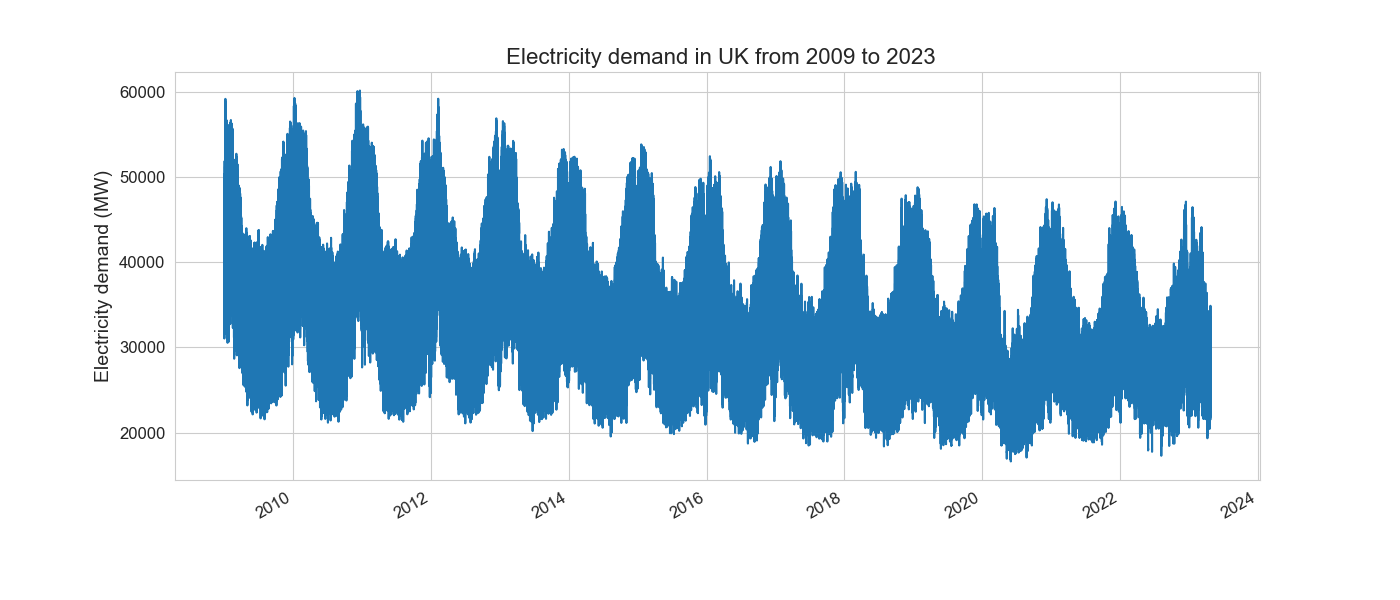
\includegraphics[width = \textwidth]{imagenes/TimeSeries.png}
    \caption{Serie temporal con tiempo discreto }\label{fig:TimeSeries}
\end{figure}
\end{center}




Se supone que cada observación $x_t$ es una realización de cierta variables aleatoria $X_t$. Una serie temporal $\{x_t, \, t \in T_0\}$ es una realización de una familia de variables aleatorias $\{X_t, \, t \in T_0\}$. Estas consideraciones sugieren modelar los datos como una realización (o parte de una realización) de un proceso estocástico $\{X_t, \, t \in T\}$ con $T_0 \subseteq T$.

\begin{definition}
    Un proceso estocástico es una familia de variables aleatorias $\{X_t, \, t \in T\}$ definidas en el espacio de probabilidad $(\Omega, \mathcal{F}, P)$.
\end{definition}

En el análisis de series temporales el conjunto de índices $T$ es un conjunto de puntos, normalmente $\{0, \pm1, \pm2, \dotsc, \}$, $\{1,2,3,\dotsc\}$, $[0, \infty)$ o $(-\infty, \infty)$. Aunque también se puede definir procesos estocásticos en los cuales $T$ no es un subconjunto de $\mathbb{R}$.



\begin{remark}
    El término serie temporal se usa frecuentemente para referirse tanto a los datos como al proceso del cual es una realización.
\end{remark}


\subsection{Modelos estacionarios y estrictamente estacionarios}
A la hora de estudiar un número finito de variables, lo más común es usar la matriz de covarianzas para obtener información sobre la dependencia entre ellas. En el caso de las series temporales, es necesario extender este concepto para tratar con conjuntos infinitos de variables aleatorias. En este caso se utliza la función de covarianzas.

\begin{definition}
    Si $\{X_t, \, t\in T\}$ es un proceso estocástico tal que $E(X_t^2)<\infty$ para todo $t\in T$, entonces la función de autocovarianzas $\gamma_X(\cdot, \cdot)$ de $\{X_t\}$ se define como
    \begin{equation}\label{eq:fun_autocov}
        \gamma_x(r,s) = Cov(X_r, X_s) = E[(X_r - E[X_r])(X_s-E[X_s])], \quad r,s \in T.
    \end{equation}
\end{definition}


\begin{definition}
     Si $\{X_t, \, t\in T\}$ es un proceso estocástico tal que $E(X_t^2)<\infty$, entontes
     \begin{enumerate}
         \item La función de autocorrelación simple (fas) se define como
         \begin{equation}\label{eq:ACF}
             \rho(r,s) = \frac{Cov(X_r, X_s)}{\sqrt{Var(X_r)(Var_s)}} = \frac{\gamma(r,s)}{\sqrt{\gamma(r,r) \gamma(s,s)}}.
         \end{equation}
         \item La función de autocorrelación parcial (fap) se define como
         \begin{equation}\label{eq:PACF}
             \alpha(r,s) = Corr(X_r, X_s \;\mid\; X_{r+1}, X_{r+2}, \dotsc, X_{s-1}) \quad \forall r < s.
         \end{equation}
     \end{enumerate}
\end{definition}

\begin{definition}\label{def:stationarity}
    Una serie temporal $\{X_t,\, t \in \mathbb{Z}\}$ se dice que es estacionaria si 
    \begin{enumerate}
        \item $E[X_t^2] <\infty$ $\forall t \in \mathbb{Z}$
        \item $E[X_t] = \mu$ $\forall t \in \mathbb{Z}$
        \item $\gamma_X(r,s) = \gamma_X(r+t, s+t)$ $\forall r,s,t \in \mathbb{Z}.$
    \end{enumerate}
\end{definition}

Esta definición de estacionaridad es referida habitualmete como estacionaridad débil. En este trabajo el término de estacionaridad se referirá siempre a la Definición \ref{def:stationarity}.


\begin{figure}
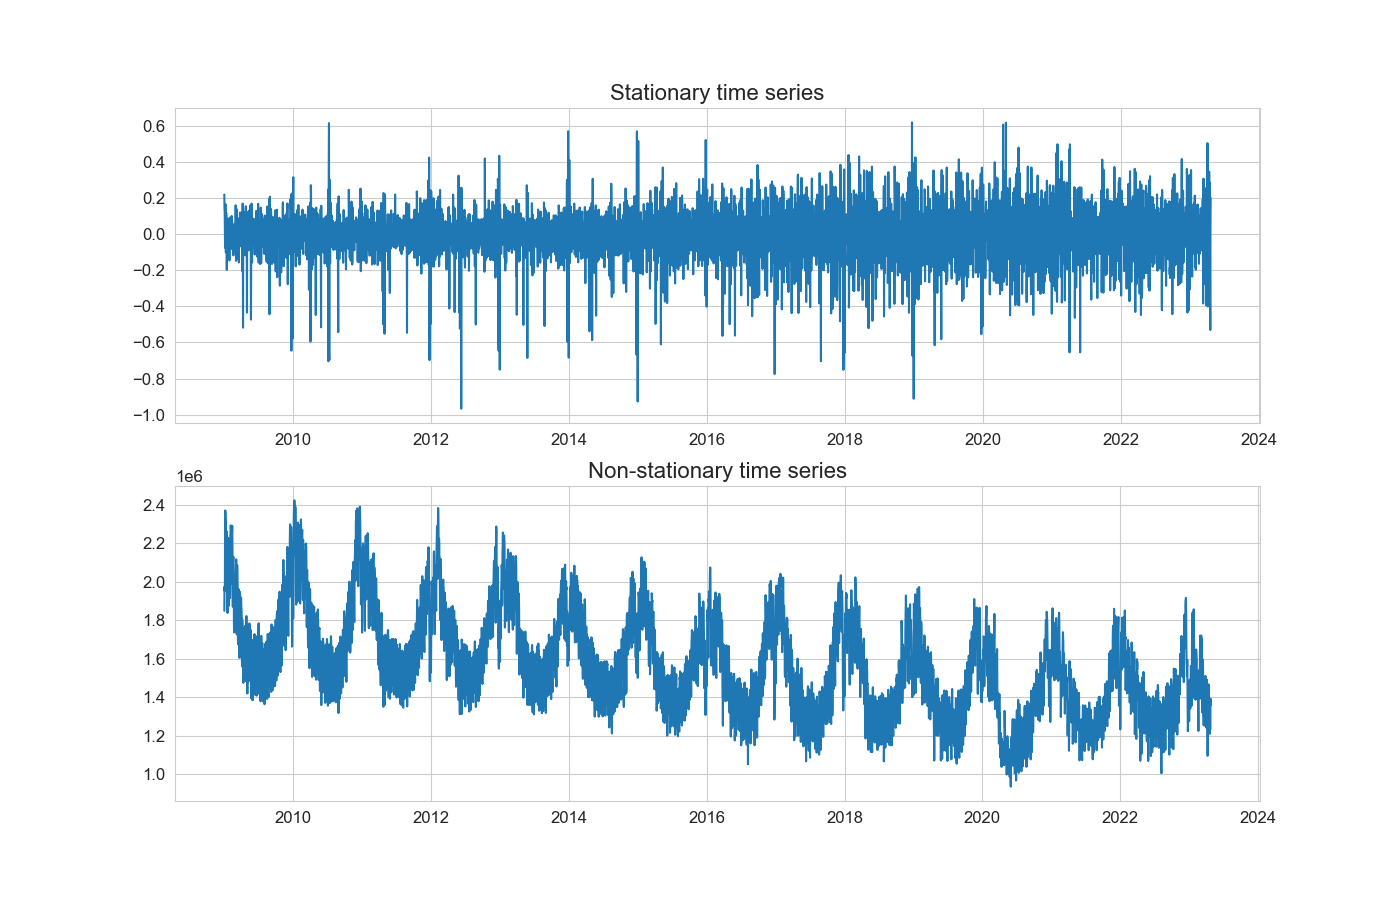
\includegraphics[width = \textwidth]{imagenes/Stationarity.png}
\caption{Ejemplos de serie estacionaria y no estacionaria, respectivamente.}\label{fig:Stationarity}
\end{figure}

La Figura 2 muestra dos ejemplos de series temporales: una estacionaria y otra no estacionaria. En el primer gráfico se observa que la media es cero y la varianza es constate, como dice la Definición \ref{fig:Stationarity}. Por otro lado, en la segunda gráfica se ve que a lo largo de los años la media disminuye y hay patrones de repetición, es decir la media y la varianza no son constantes.


\begin{remark}
    Si $\{X_t, \,t \in \mathbb{Z}\}$ es estacionaria entonces $\gamma_X(r,s) = \gamma_X(r-s,0)$ para todo $r,s \in \mathbb{Z}$. Por tanto, es conveniente redifinir la función de autocovarianzas de un proceso estacionario como la función de una sola variable,
    \begin{equation*}
        \gamma_X(h) = \gamma_X(h,0) = Cov(X_{t+h}, X_t) \quad \text{para todo } t,h \in \mathbb{Z}.
    \end{equation*}
La función $\gamma_X(\cdot)$ hace referencia a la función de autocovarianzas de $\{X_t\}$ y $\gamma_X(h)$ a su valor para el retardo $h$. La función de autcorrelación simple de $\{X_t\}$ se define de forma análoga como función de un solo valor para el retardo $h$,
\begin{equation*}
    \rho_X(h) := \frac{\gamma_X(h)}{\gamma_X(0)} = Corr(X_{t+h}, X_t) \quad \forall t,h \in \mathbb{Z}.
\end{equation*}
\end{remark}

\begin{remark}
    La definición de estacionaridad se ha dado para el caso en que $T = \mathbb{Z}$. No es difícil definir la estacionaridad usando un conjunto de índices más general, pero en este caso, no es necesario extender la definición. Si se quiere modelar un conjunto de datos $\{x_t, \, t\in T \subset \mathbb{Z}\}$ como una realización de un proceso estacionario, se puede considerar como parte de una realización de un proceso estacionario $\{X_t, \, t \in \mathbb{Z}\}$.
\end{remark}

\begin{definition}[Estacionaridad estricta]\label{def:strictly_stationary}
    Una serie temporal $\{X_t, \,t \in \mathbb{Z}\}$ se dice estrictamente estacionaria si las distribuciones conjuntas $(X_{t_1}, \dotsc, X_{t_k})$ y $(X_{t_1+h}, \dotsc, X_{t_k+h})$ son la misma para todos los enteros positivos $k$ y para todo $t_1, \dotsc, t_k \in \mathbb{Z}$. 
\end{definition}

Si $\{X_t\}$ es estrictamente estacionaria, tomando $k=1$ en la Definición \ref{def:strictly_stationary} se tienen que $X_t$ tiene las misma distribución para todo $t \in \mathbb{Z}$. En particular, si $E[X_t^2] < \infty$, se tiene que $E[X_t]$ y $Var[X_t]$ son constantes. Además, para $k=2$ se tiene que $X_{t+h}$ y $X_t$ tienen la misma distribución conjunta para todo $h\in\mathbb{Z}$. Por tanto, la estacionaridad estricta implica estacionaridad (débil).

% \begin{proposition}
%     Sea $\gamma(\cdot)$ la función de autocovarianza de un proceso estacionario $\{X_t, \; t \in T\}$, entonces se cumple:
%     \begin{enumerate}
%         \item $\gamma(0) \geq 0$.
%         \item $\abs{\gamma(h)} \leq \gamma(0)$, para todo $t\in T$.
%         \item $\gamma(h) = \gamma(-h)$, para todo $t\in T$.
%         \item $\gamma(\cdot)$ es definida no negativa, es decir, $\sum_{i,j=1}^n a_i \gamma(i-j) a_j \geq 0$ para $n\in \mathbb{N}$ y $(a_1, a_2, \dotsc, a_n)\in \mathbb{R}^n$.
%     \end{enumerate}
%     \begin{proof}
%         \begin{enumerate}
%             \item $\gamma(0) = Cov(X_t, X_t) = Var(X_t) \geq 0.$
%             \item Por la desigualdad de Cauchy-Schwarz...
%             \item $\gamma(-h) = Cov(X_{t-h}, X_t) = Cov(X_t, X_{t+h} = \gamma(h)$.
%             \item ...
            
%         \end{enumerate}
%     \end{proof}
% \end{proposition}





\subsection{Descomposición de una serie temporal}
En el método de descomosición clásica, los datos se generan como la suma de tres efectos,
\begin{equation}\label{eq:descom}
    X_t = \mu_t + S_t + Y_t,
\end{equation}
donde $\mu_t$ es el \emph{nivel de la serie} o \emph{componente de tendencia}, $S_t$ es conocido como el \emph{componente estacional} y, por último, $Y_t$ es el componente puramente aleatorio o \emph{innovación}. En el caso de no presentar componente estacional, la descomposición se reduce a 
\begin{equation}\label{eq:descom2}
    X_t = \mu_t + Y_t.
\end{equation}

En la Figura \ref{fig:Decomposition} se muestra la decomposición aditiva  de los datos. Habitualmente, el nivel $\mu_t$ se modela mediante un polinomio del tiempo de orden menor o igual a dos, y la estacionalidad como una función periódica, que verifica la condición
\begin{equation*}
    S_t = S_{t-s},
\end{equation*}
donde $s$ es el periodo de la función. Una serie mensual con estacionalidad anual tiene periodo $s=12$ meses, ya que se supone que los \emph{coeficientes estacionales}, $S_t$, se repiten cada $12$ observaciones y una serie diaria con estacionalidad semanal tiene $s=7$ días.

La innovación es un componente aleatorio que recoge todos los demás efectos que actúan sobre la serie. Se supone que las variables aleatorias $Y_t$ tienen una estructura estable a lo largo del tiempo: media cero, varianza constante y distribución normal. Además, las observaciones correspondientes a dos periodos distintos de tiempo son independientes, es decir, conocer el valor $Y_t$ no proporciona ninguna información sobre el posible valor de $Y_{t+1}$.



\begin{figure} 
    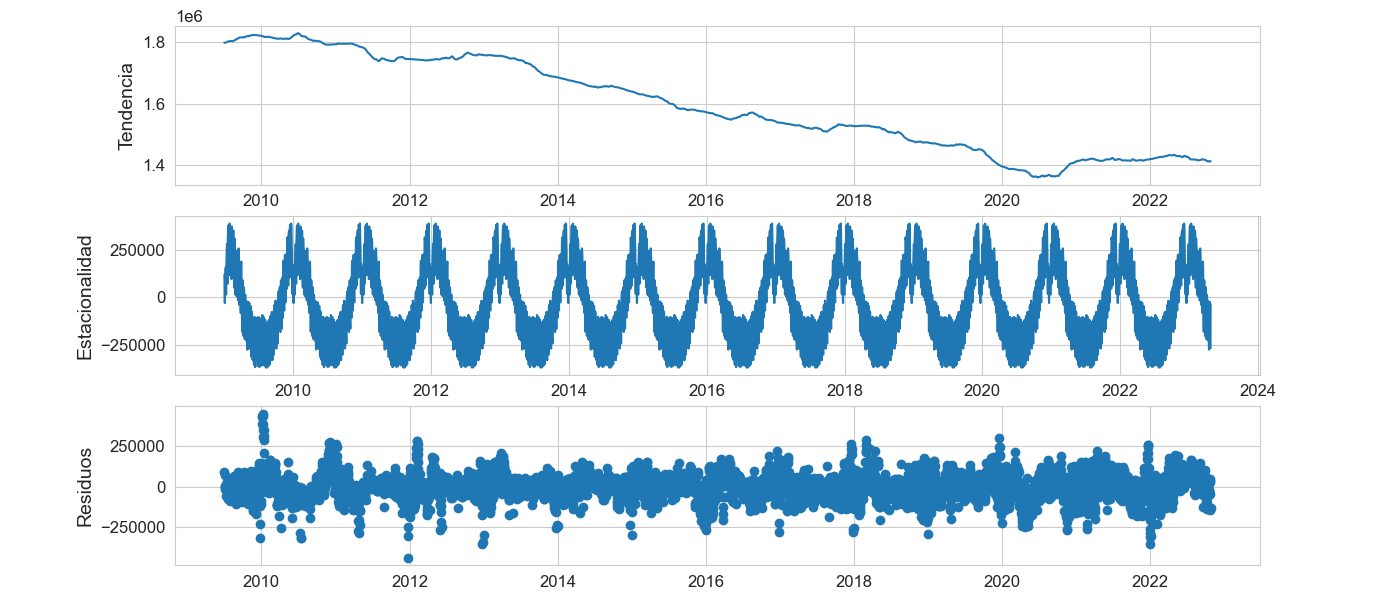
\includegraphics[width = \textwidth]{imagenes/Decomposition.png}
    \caption{Descomposición aditiva de los datos}\label{fig:Decomposition}
\end{figure}



Una alternativa a esta descomposición es la descomposición multiplicativa, que consta de los mismos componentes, y también es muy utlizada, 
\begin{equation}\label{eq:descom3}
    X_t = \mu_t \times S_t \times Y_t.
\end{equation}

% \begin{figure}
%     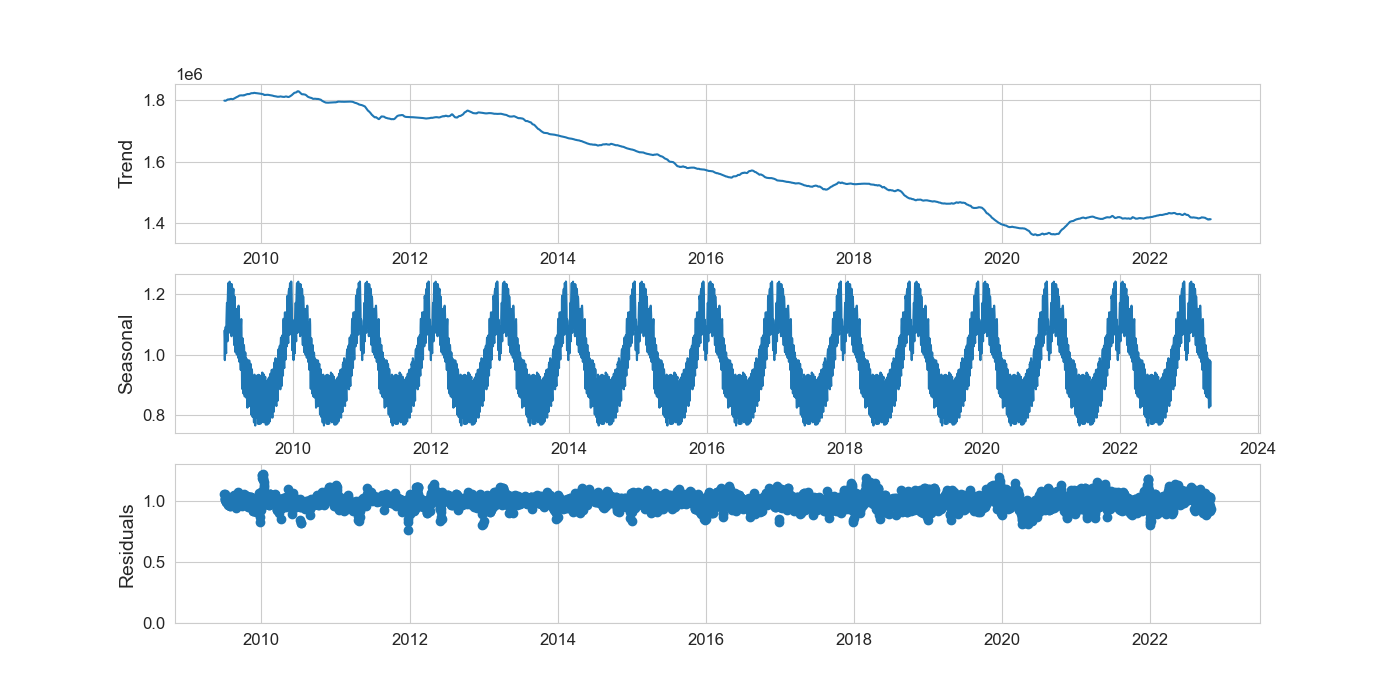
\includegraphics[width = \textwidth]{imagenes/Decomposition2.png}
%     \caption{Descomposición multiplicativa de los datos}\label{fig:Decomposition2}
% \end{figure}


\newpage
\section{Procesos autoregresivos y de media móvil}
En esta sección se estudia una clase muy importante de series temporales, definida en términos de ecuaciones en diferencias lineales con coeficientes constantes. La imposición de esta estructura adicional define una familia de procesos estacionarios, los llamados procesos de media móvil autoregresivos o ARMA. Antes de estudiar dichos procesos, es necesario introducir un nuevo tipo de proceso, el proceso de ruido blanco.


\begin{definition}\label{def:WN_process}
    El proceso $\{Y_t\}$ se conoce como proceso de ruido blanco con media $0$ y varianza $\sigma^2$,
    \begin{equation} \label{eq:WN_process}
        \{Y_t\} \sim \text{WN}(0, \sigma^2),
    \end{equation}
    si $\{Y_t\}$ tiene media $0$ y función de autocovarianza
    \begin{equation} \label{eq:WN_autocov}
        \gamma(h) = 
        \left\{ \begin{array}{ll} 
        \sigma^2 & \text{si } h=0 \\
        0 & \text{si } h \neq 0 
        \end{array} \right.
    \end{equation}

    Si las variables aleatoria $Y_t$ son independiente e identicamente distribuidas con media $0$ y varianza $\sigma^2$, entonces se conocen como
    \begin{equation} \label{eq:IDD_process}
        \{Y_t\} \sim \text{IID}(0, \sigma^2).
    \end{equation}
\end{definition}

Los procesos de ruido blanco permiten generar una clase muy amplia de procesos estacionarios gracias a ecuaciones en diferencias lineales.

\begin{definition}\label{def:ARMA}
    El proceso $\{X_t, \,t\in T\}$ se dice $\arma(p,q)$ si es estacionario y para todo $t$, 
    \begin{equation}\label{eq:ARMA}
        X_t - \phi_1X_{t-1}-\dotsb-\phi_pX_{t-p} = Y_t +\theta_1Y_{t-1} + \dotsb + \theta_q Y_{t-q},
    \end{equation}
    donde $\{Y_t\}\sim \wn$. Se dice que $\{X_t\}$ es un proceso $\arma(p,q)$ con media $\mu$ si $\{X_t - \mu\}$ es un proceso $\arma(p,q)$.
\end{definition}

La ecuación \eqref{eq:ARMA} puede escribirse de forma más compacta, introduciendo la notación del operador de retardo.

\begin{definition}\label{def:lag_operator}
    Se llama operador de retardo a $B$, definido por  
    \begin{equation}\label{eq:lag_operator}
    BX_t = X_{t-1}.
\end{equation}
Además cumple las propiedades siguientes:
\begin{enumerate}
    \item $B\mu = \mu$, para $\mu$ constante.
    \item $B a X_t = a B x_t = aX_{t-1}$, para $a$ constante.
    \item Es lineal, es decir, $B(af(t) + bg(t)) = af(t-1) + b g(t-1)$.
    \item $B^kX_t = \underbrace{B\cdots B}_k X_t = X_{t-k}$.
\end{enumerate}
\end{definition}

Utilizando la notación del operador de retardo, la ecuación \eqref{def:ARMA} puede escribirse como
\begin{equation}\label{eq:ARMA_lag_op}
    \phi(B)X_t = \theta(B)Y_t,
\end{equation}
donde $\phi(B)$ y $\theta(B)$ son polinomios de grado $p$ y $q$ en el operador de retardo,
\begin{align}
    \phi(B) =& \;1 - \phi_1 B - \dotsb - \phi_p B^p \label{eq:ar_lag_op}, \\
    \theta(B) =&\; 1 +\theta_1 B + \dotsb + \theta_q B^q \label{eq:ma_lag_op}.
\end{align}

A $\phi(B)$ se le conoce como el operador del proceso autoregresivo u operador AR y a $\theta(B)$ se le conoce como el operador del proceso de media móvil u operador MA. El proceso $\arma(p,q)$ es estacionario si, y solo si, el módulo de las raíces de $\phi_p(B) = 0$ son mayores a $1$.

Para cualquien función de autocovarianza $\gamma(\cdot)$ tal que $\lim_{h\rightarrow\infty} \gamma(h) = 0$, y para todo entero $k>0$, es posible encontrar un proceso ARMA con función de autocovarianza $\gamma_x(h) = \gamma(h)$ $h=0,1\dotsc,k$. Por razones como esta, la familia de los procesos ARMA juega un papel muy importante en la modelación de series temporales. Además, su estrucutura lineal conduce a un teoria simple de predicciones lineales.

\begin{example}[Proceso $\ma(q)$]
    Si $\phi(B) \equiv 1$, entonces
    \begin{equation}\label{eq:ma_process}
        X_t = \theta(B)Y_t,
    \end{equation}
    y a este proceso se le conoce como proceso de media móvil de orden $q$ o $\ma(q)$ por sus siglas en inglés, \emph{moving average}. Se tiene que $\{X_t\}$ es estacionaria ya que, tomando $\theta_0 = 1$ y $\theta_j = 0$ para $j > q$, se tiene que, $\forall h > 0$
    \begin{align*}
        E[X_t] & = \sum_{j=0}^q \theta_j E[Y_{t-j}] = 0 \quad \text{y}\\
        \gamma_X(h) = Cov(X_{t+h}, X_t) & = \left\{\begin{array}{ll}
            \sigma^2 \sum_{j=h}^{q} \theta_j \theta_{j - h} & \text{si } h \leq q,  \\
            0 & \text{si } h > q.
        \end{array}\right.
    \end{align*}
\end{example}

\begin{example}[Proceso $\ar(p)$] Si $\theta(B)\equiv1$, entonces
\begin{equation}\label{eq:ar_process}
    \phi(B)X_t = Y_t
\end{equation}
y a este proceso se le conoce como proceso autorregresivo de orden $p$ o $\ar(p)$. Este proceso es estacionario solo si las raíces de $\phi(B) = 0$ están fuera del cículo unidad.
\end{example}

\subsection{Procesos ARIMA y SARIMA}
Se puede definir nuevos procesos no estacionarios a partir de la Definición \ref{def:ARMA}. Para ello, se incorpora raíces unitarias al proceso ARMA a través de un operador.


\begin{definition}
    El operador de diferenciación, denotado por $\nabla$, se define como
    \begin{equation*}
        \nabla = 1 -B.
    \end{equation*}
\end{definition}

De igual modo, se define el operador de diferenciación de orden $s$ u operador de diferenciación estacional como $\nabla_s = 1 - B^s$. Con los operadores se puede definir un nuevo proceso.

\begin{definition}
    Se dice que $\{X_t\}$ es un proceso integrado de orden $h$, $I(h)$, si al diferenciar $\{X_t\}$ $h$ veces se obtiene un proceso estacionario.
\end{definition}

Uniendo los procesos estudiados, es decir los $\arma(p,q)$ con los procesos integrado, se obtiene los procesos de media móvil integrados autorregresivos o ARIMA.

\begin{definition}
    Se dice que $\{X_t\}$ es un proceso $\arima(p,d,q)$ si
    \begin{equation}\label{eq:ARIMA}
        \phi(B)(1-B)^d X_t = \theta(B) Y_t
    \end{equation}
    o, con la notación del operador de diferenciación
        \begin{equation}\label{eq:ARIMA2}
        \phi(B)\nabla^d X_t = \theta(B) Y_t,
    \end{equation}
    donde $\{Y_t\} \sim \wn$, $\theta(B) = 1 + \theta_1B + \dotsb + \theta_qB^q$, $\phi(B) = 1 - \phi_1B - \dotsb - \phi_qB^p$ y las raíces de $\phi(B) = 0$ tienen módulo mayor que 1.
\end{definition}

Por la estructura de los procesos ARIMA, se sabe que son no estacionarios, sin embargo se puede definir $W_t = \nabla^d X_t$ que es un proceso $\arma(p,q)$ y sí es estacionario. Los procesos ARIMA se pueden extender aún más introduciendo el operador de diferenciación estacional.

\begin{definition}
    $\{X_t\}$ es un proceso ARIMA multiplicativo estacional o SARIMA, denotado $\{X_t\} \sim \arima(P,D,Q)_s\times (p,d,q)$, si
    \begin{equation}\label{eq:SARIMA}
        \Phi(B^s)\phi(B) \nabla_s^D \nabla^d X_t = \theta(B) \Theta(B^s) Y_t,
    \end{equation}
    donde
    \begin{itemize}
        \item $\{Y_t\} \sim \wn$,
        \item $\nabla_s^D$ representa la diferenciación estacional,
        \item $\nabla^d$ representa la diferenciación regular
        \item $\Phi(B^s) = 1 - \Phi_1B^s - \dotsb - \Phi_PB^{sP}$ es el operador AR estacional,
        \item $\phi(B) = 1 - \phi_1B - \dotsb - \phi_pB^p$ es el operador AR,
        \item $\Theta(B^s) = 1 - \Theta_1B^s + \dotsb + \Theta_QB^{sQ}$ es el operador MA estacional,
        \item $\theta(B) = 1 + \theta_1B + \dotsb + \theta_qB^q$ es el operador MA.
    \end{itemize}
\end{definition}

La implementación en Python de este método se ha hecho con los datos diarios, ya que si se tomara el dataset completo el tiempo de ejecución ascendería hasta horas o días. La Figura \ref{fig:SARIMA} muestra tanto los datos ajustados como las predicciones. Lo que cabe destacar de esta imagen son dos cosas: la diferencia de ajuste entre el conjunto train y el conjunto test y la amplitud del intervalo de confianza. Por una parte, el modelo se ajusta correctamente a los datos, pero no capta correctamente los patrones de estacionalidad de los años del test. Se puede ver de forma más clara en la Figura \ref{eq:SARIMA} cómo no aprende correctamente de las oscilaciones anuales de los datos. Por otra parte, el intervalo de confianza del $95\%$ es muy amplio, de modo que los datos temporales obviamente vas a estar en su interior. 

De este modelo, cabe destacar que el error medio absoluto medio es del $11.58\%$ y su tiempo de ejecución es $8$ minnutos y $24$ segundos. El error no es significativamente grande, pero el mayor inconveniente es que no es capaz de modelar correctamente los cambios estacionales, ya que esta es un factor crucial en el análisis de series temporales.

El mayor inconveniente de los modelos SARIMA es ajustar los datos y entontrar los valores óptimos de  $p$, $q$, $P$ y $Q$. En este caso se ha utlizado la metodología de Box-Jenkins para encontrar dichos valores. En este caso, el modelo mostrado en las Figuras \ref{fig:SARIMA} y \ref{fig:SARIMA_pred} se corresponde con un modelo $\arima(3,1,2)_{12}\times(7,1,7)$. A la hora de encontrar los modelos idóneos para los datos presentados es necesario ajustar muchos modelos para diferentes valores de los parámetros que propone el analista y, teniendo en cuenta que el algoritmo tarda unos $10$ minutos por cada modelo, el tiempo de computación y de búsqueda es demasiado grande. Una alternativa a buscar manualmente los valores es introducir una lista de posibles modelos en el programa y escoger aquel que minimice el error, sin embargo, así aumenta el coste computacional.

En consecuencia, el modelo SARIMA funciona correctamente, pero existen otros modelos con menor coste computacional que podrían ajustar lo datos de forma más precisa. En las siguientes secciones se presenta algunos de esos métodos.




\begin{center}
\begin{figure}[h]
    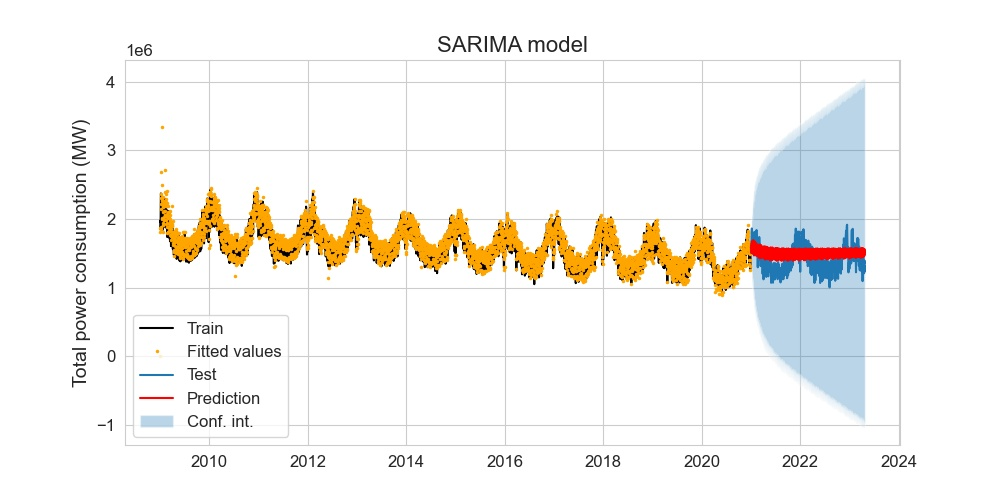
\includegraphics[width = \textwidth]{imagenes/SARIMA.jpg}
    \caption{Modelo ajustado con SARIMA}\label{fig:SARIMA}
\end{figure}
\end{center}

\begin{center}
\begin{figure}[h]
    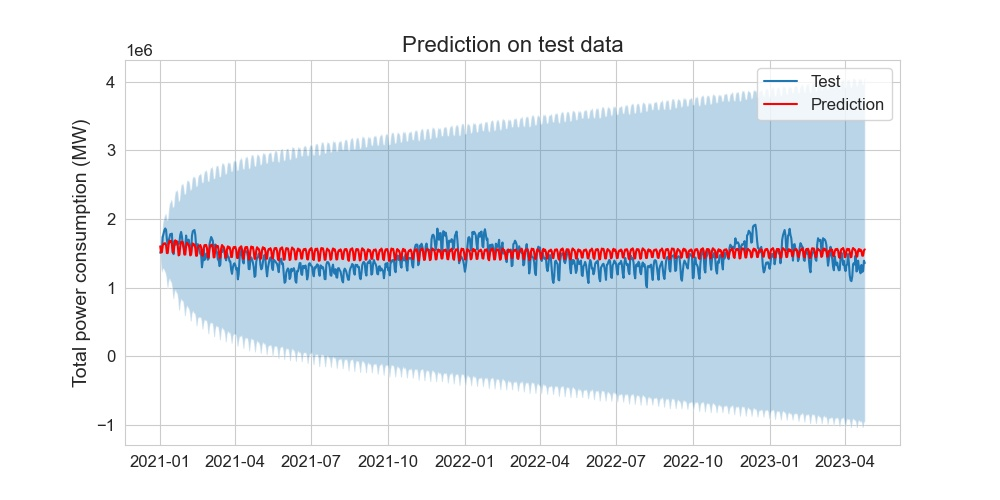
\includegraphics[width = \textwidth]{imagenes/SARIMA_pred.jpg}
    \caption{...}\label{fig:SARIMA_pred}
\end{figure}
\end{center}






\newpage
\section{Suavizado exponencial}

El suavizado exponencial o alisado exponencial describe una clase de métodos de predicción. De hecho, muchos de los métodos de predicción más exitosos estan basandos en el concepto del suavizado exponencial. Hay una gran variedad de métodos basados en esta familia, cada una con la propiedad de que los pronósticos son combinaciones ponderadas de observaciones pasadas, donde las observaciones recientes tienen  más peso que las observaciones más alejadas. El nombre ``suavizado exponencial'' refleja el hecho de que los pesos caen exponencialmente según las observaciones son más lejanas.

En este capítulo se va a estudiar tres de los métodos más reconocidos en la familia de suavizado exponencial: el método de suavizado simple, el método lineal de Holt y el método de Holt-Winters. Todos estos algoritmos están implementados en Python en el paquete \emph{statsmodels}.




\subsection{Suavizado exponencial simple}
El modelo de suavizado exponencial simple recibe su nombre por ser el más secillo de esta familia. Esta técnica solo se puede aplicar a datos que no presentan tendencia ni patrones estacionales. 

El método de \textit{simple exponential smoothing}, resultado del trabajo de Brown en la decada de los 50s, toma la predicción del periodo previo y lo ajusta usando el error de predicción.

Si se supone que se dispone de las observaciones hasta $t-1$ y se quiere predecir el próximo valore de la serie temporal, $X_t$. Cuando se dispone de la observación $X_t$, el error de la predicción se calcula como $X_t - \hat{X}_t$, donde $\hat{X}_t$ es la predicción. La predicción para el siguiente tiempo se define como
\begin{equation} \label{eq:simple_exp}
   \hat{X}_{t+1} = \hat{X}_t + \alpha (X_t - \hat{X}_t), 
\end{equation}

donde $\alpha$ es una constante entre $0$ y $1$.

Se puede ver que la nueva predicción es la predicción anterior sumando un ajuste para el error de la última predicción. Cuando $\alpha$ tiene un valor cercano a $1$, la nueva predicción tendrá un ajuste significativo por el error en la anterior predicción. Por el contrario, cuando $\alpha$ es cercano a $0$, el nuevo pronóstico tendrá un ajuste muy pequeño.

Otra forma de escribir la ecuacion \eqref{eq:simple_exp} es
\begin{equation} \label{eq:simple_exp2}
    \hat{X}_{t+1} = \alpha X_t + (1-\alpha)\hat{X}_t. 
\end{equation}

La predicción $\hat{X}_{t+1}$ está basada en la ponderación de la observación más reciente, $X_t$, con un peso de $\alpha$ y la predición más reciente, $\hat{X}_t$ con peso de $1-\alpha$. Las implicaciones del suavizado exponencial se pueden observar más fácilmente si se expande la ecuación \eqref{eq:simple_exp2} sustituyendo $\hat{X}_t$ por sus componentes, como sigue:


\begin{equation*}
\begin{split}
\hat{X}_{t+1} & =  \alpha X_t + (1-\alpha) [\alpha X_{t-1} + (1-\alpha)\hat{X}_{t-1}] \\
& = \alpha t_t + \alpha(1-\alpha)X_{t-1} + (1-\alpha)^2\hat{X}_{t-1}.
\end{split}
\end{equation*}

Si se repite este proceso de sustitución de $\hat{X}_{t-1}$ por sus componentes, $\hat{X}_{t-2}$ por sus componentes, y así, se llega al resultado

\begin{equation*}
\begin{split}
    \hat{X}_{t+1} = &\; \alpha X_t + \alpha(1-\alpha)X_{t-1} + \alpha(1-\alpha)^2X_{t-2} + \alpha(1-\alpha)^3X_{t-3} \\
    & + \alpha(1-\alpha)^4X_{t-4} + \dotsb +  \alpha(1-\alpha)^{t-1}X_1 + (1-\alpha)^t\hat{X}_1.
\end{split}
\end{equation*}

Por tanto $\hat{X}_{t+1}$ representa un proceso de media móvil ponderado con todas las observaciones pasadas y los pesos decreciendo exponencialmente, de ahí el nombre de ``suavizado exponencial''.

La limitación de este método es que no puede modelar datos que presentan tendencia o componente estacional. Para aplicar este algoritmo se ha eliminado dichas componentes de los datos. En  la Figura \ref{fig:SimpleES1} se puede ver cómo el modelo ajusta a los datos, pero las predicciones son estáticas en el tiempo, con lo que no se ajusta correctamente a los posibles cambios de los datos.

\begin{figure}[h]
    \centering
    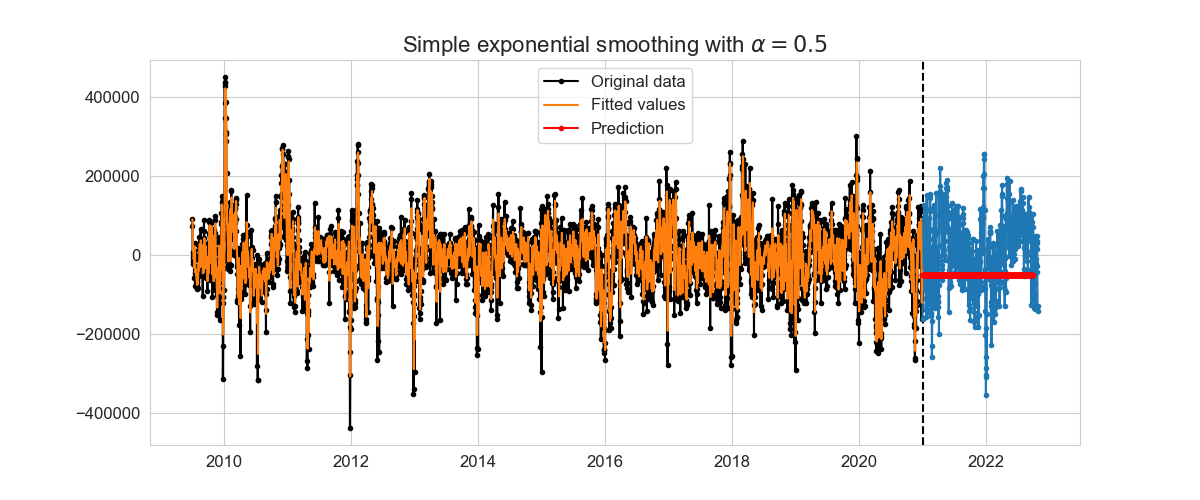
\includegraphics[width = 0.95\textwidth]{imagenes/SimpleES1.png}
    \caption{Valores ajustados y predicción de método de suavizado exponencial simple}\label{fig:SimpleES1}
\end{figure}


En la Figura \ref{fig:SimpleES2} se presentan tres modelos, en los dos primeros se fija el valor de $\alpha$ como $0.2$ y $0.6$, respectivamente, y el tercer modelo busca el valor óptimo. Se observa en el gráfico que todas las predicciones son estáticas y, en la Tabla \ref{tab:simple_exp}, se ve que el error absoluto medio porcentual asciende hasta el $450\%$. El error alcanza valores tan altos porque los datos son cercanos a cero, es decir, al dividir por dichos valores, el error incrementa rápidamente. Por esta razón, en este caso, también se ha estudiado la suma de los errores al cuadrado (SSE). La tabla muestra que, efectivamente, el menor valor de SSE se alcanza para el valor de $\alpha$ que ha sido optimizado. Sin embargo, el ajuste de las predicciones no es lo suficiente preciso.



\begin{figure}[h]
    \centering
    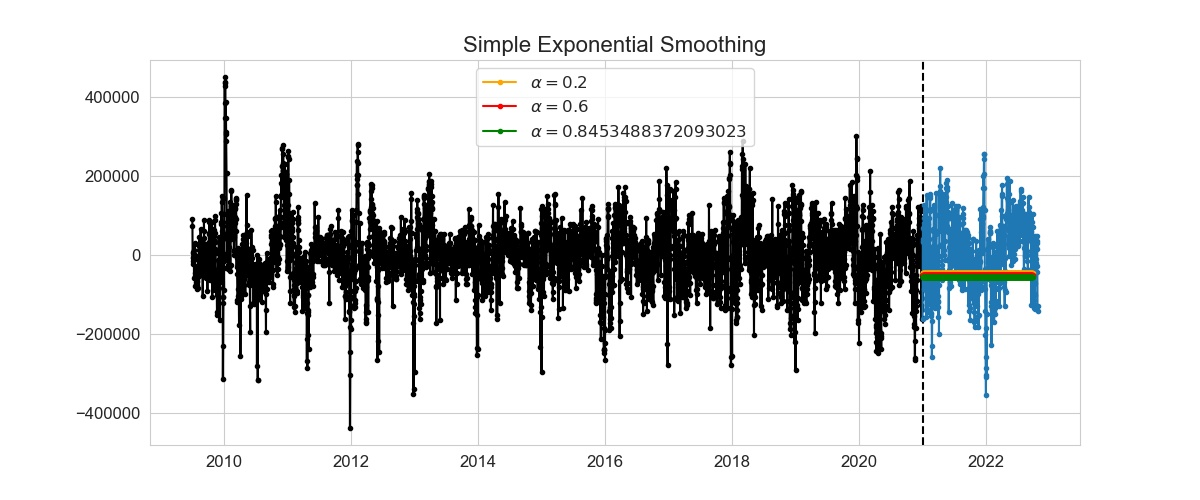
\includegraphics[width = 0.95\textwidth]{imagenes/SimpleES2.jpg}
    \caption{Modelos del método de suavizado exponencial simple con diferentes parámetros de suavizado}\label{fig:SimpleES2}
\end{figure}

\begin{table}[h] 
\centering
\begin{tabular}{cccc} \hline
     & Modelo 1 & Modelo 2 & Modelo 3  \\ \hline
    $\alpha$ &  $0.2$ &   $0.6$ &   $0.8453488$ \\ 
      % $l_0$ &   $59316.54$ &  $59316.54$ &   $59316.54$ \\ 
      MAPE & $382.808$	 &   $423.329$ &  $456.399$ \\
      SSE & $1.6106\cdot 10^{13}$ & $1.2314\cdot 10^{13}$ & $1.19017\cdot 10^{13}$ \\
      Tiempo (s) & $0.029$ &   $0.033$ &  $0.045$ \\ \hline
\end{tabular}
\caption{Parámetros, tiempo y error del método de suavizado exponencial simple} \label{tab:simple_exp}
\end{table}



\newpage
\subsection{Método lineal de Holt}
Holt extendió el suavizado exponencial simple al suavizado exponencial lineal para permitir el pronósticos con datos que presentan tendencias. La predicción de método lineal de Holt se basa en utilizar dos constantes $\alpha$ y $\beta^*$ (con valores entre $0$ y $1$), y tres ecuaciones
\begin{align}
    \text{Nivel:} \quad& l_t = \alpha X_t + (1-\alpha)(l_{t-1} + b_{t-1}),\label{eq:Holt:nivel}\\
    \text{Crecimiento:} \quad& b_t = \beta^*(l_t - l_{t-1}) + (1-\beta^*)b_{t-1},\label{eq:Holt:crec}\\
    \text{Predicción:} \quad& \hat{X}_{t+h \mid t} = l_t + b_th.\label{eq:Holt:pred}
\end{align}

$l_t$ denota una estimación del nivel de la serie en el instante $t$ y $b_t$ denota una estimación de la pendiente (o crecimiento) de la serie en el instante $t$.


La ventaja de este modelo es que puede trabajar con datos con tendencia, por ello, se ha transformado los datos eliminando la componente estacional, para así aplicar este método.

La Figura \ref{fig:Holt1} muestra los valores ajustados y la predicción del modelos lineal de Holt para los valores $\alpha=0.5$ y $\beta^* = 0.2$. Sin embargo, se observa como el valor de la predicción desciende, alejándose de los valores reales.

A continuación se ha probado tres modelos con las opciones disponibles de Python. El primer modelo es el presentado por las ecuaciones \eqref{eq:Holt:nivel}, \eqref{eq:Holt:crec} y \eqref{eq:Holt:pred}. El segundo modelo ajusta la tendencia usando un modelo multiplicativo, en lugar de usar el modelo aditivo presentado. Por último, el tercer modelo presenta el método amortiguado del método de Holt. En este modelo las ecuaciones consideran un nuevo parámetro de amortiguamiento, $\phi$.

Todos los modelos optimizan los valores de $\alpha$ y $\beta^*$, se puede ver los parámetros escogido en la Tabla \ref{tab:holt}. Los modelos se ejecutan en menos de un segundo, por tanto el tiempo de computación no es un problema en este caso. Sin embargo, en la Figura \ref{fig:Holt2} se observa cómo los modelos uno y dos se alejan de los valores reales del test y no predicen correctamente. El modelo amortiguado es el único que ofrece una predicción coherente con los datos presentados. La Tabla \ref{tab:holt} muestra que el error absoluto medio pocentual se minimiza en el modelo amortiguado con un valor del $7\%$.




\begin{figure}[h]
    \centering
    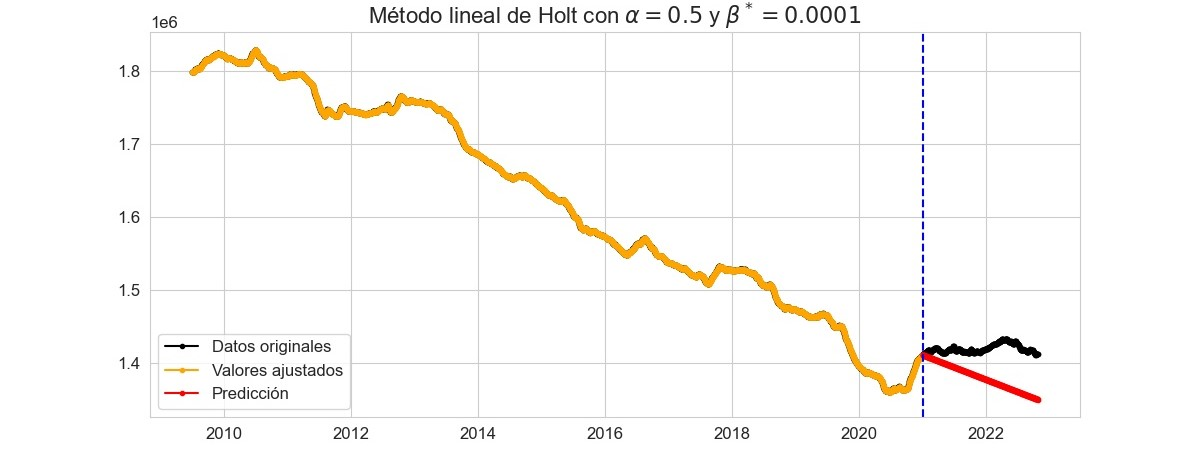
\includegraphics[width = \textwidth]{imagenes/Holt1.jpg}
    \caption{Valores ajustados y predicción del modelo lineal de Holt}\label{fig:Holt1}
\end{figure}


\begin{figure}[h]
    \centering
    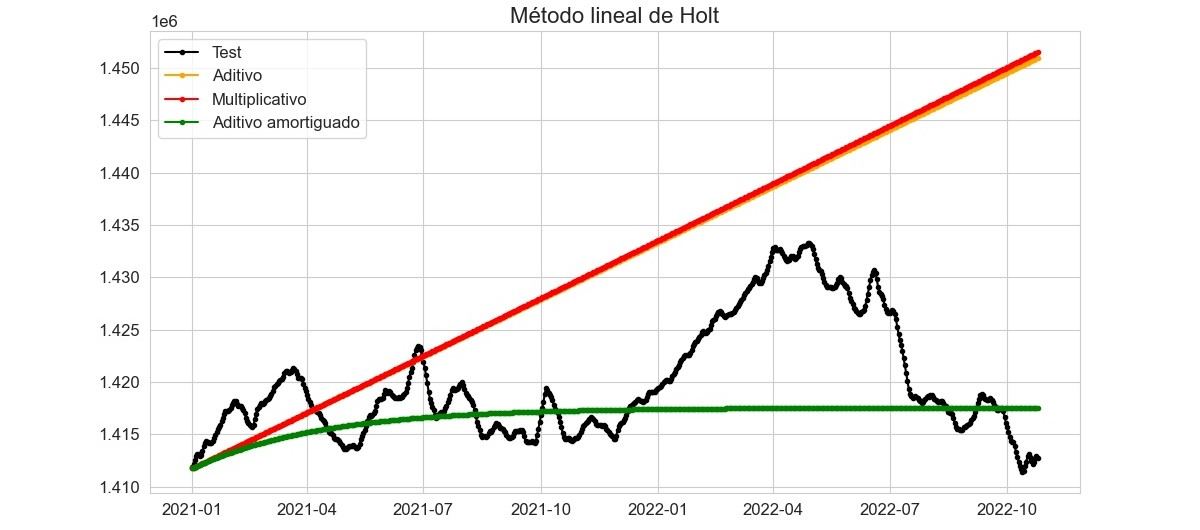
\includegraphics[width = \textwidth]{imagenes/Holt2.jpg}
    \caption{Predicciones de tres modelos con el método lineal de Holt}\label{fig:Holt2}
\end{figure}


\begin{table}[ht] 
\centering
\begin{tabular}{cccc}  \hline
     & Aditivo & Multiplicativo & Amortiguado  \\ \hline
    $\alpha$ &  $0.85357$ &   $0.85357$ &   $0.877149$ \\ 
    $\beta$ &  $0.021886$ &   $0.02188$ &   $0.0001$ \\ 
    $\phi$ &  - &   - &   $0.99$ \\ 
    % $l_0$ &   $1847570$ &  $1847570$ &   $1847570$ \\ 
    % $b_0$ &   $39474.44$ &  $39474.44$ &   $39474.44$ \\ 
      MAPE & $23.202$	 &   $10.671$ &  $7.031$ \\
      Tiempo (s) & $0.515$ &   $0.684$	 &  $0.598$ \\ \hline
\end{tabular}
\caption{Parámetros, error y tiempo del método de Holt} \label{tab:holt}
\end{table}

\newpage
\subsection{Algoritmo de Holt-Winthers}
Holt y Winters extendieron el método de Holt para incorporar el componente estacional. El método de Holt-Winters consta de tres ecuaciones de suavizado: una para el nivel $l_t$, otra para la tendencia $b_t$ y la última para el componente estacional $s_t$. A cada ecuación le corresponde un parámetro de suavizado $\alpha$, $\beta^*$ y $\gamma$, respectivamente.
\begin{align*}
    \text{Nivel:} \quad& l_t = \alpha(X_t - s_{t-s}) + (1-\alpha)(l_{t-1} + b_{t-1}),\\
    \text{Crecimiento:} \quad& b_t = \beta^*(l_t - l_{t-1}) + (1-\beta^*)b_{t-1},\\
    \text{Estacionalidad:} \quad& s_t = \gamma (X_t  - l_{t-1} - b_{t-1}) + (1-\gamma)s_{t-s},\\
    \text{Predicción:} \quad& \hat{X}_{t+h\mid t} = l_t + b_th + s_{t+h-s(k+1)},
\end{align*}

donde $s$ es el periodo de estacionalidad y  $k = \lfloor (h-1)/m \rfloor$, lo que asegura que las estimaciones de los índices estacionales utilizados para la predicción provienen del último año de la muestra.

A continuación, se van a presentar modelos del algorimo de Holt-Winters aplicados a los datos medidos diaramente y a los datos completos. La Figura \ref{fig:HoltWinters1} muestra cómo tanto los valores ajustados como las predicciones se ajustan a los valores reales de la serie. Al igual que con los otros modelos, se ha implementado las opciones disponibles, ajustado hasta cuatro modelos distintos que aplican el algoritmo de forma aditiva y multiplicativa y a su vez añadiendo o no el parámetro de amortiguamiento. En todos los métodos el algoritmo busca los parámetros óptimos. Los parámetros y resultados se pueden observar en la Tabla \ref{tab:holtwinters}. Se ve que el modelo que minimiza el MAPE es el multiplicativo, con un valor del $17\%$


\begin{table}[h] 
\centering
\begin{tabular}{ccccc}  \hline
     & Aditivo & Multiplicativo & Ad. amortiguado & Mul. Amortiguado  \\ \hline
    $\alpha$ &  $0.6060$ &   $0.995$  &  $0.6060$ &   $0.995$ \\ 
    $\beta$  &  $0.0001$ &   $0.0001$ &  $0.0001$ &  $0.0001$ \\ 
    $\gamma$ &  $0.3939$ & 	 $0.005$  &	 $0.3939$ &   $0.005$ \\
    $\phi$   &     -     &       -    &    $0.99$ &    $0.99$ \\ 
    % $l_0$    & $1798649$ &  $1798649$ & $1798649$ & $1798649$ \\ 
    % $b_0$    &  $177.84$ &  $177.84$ &  $177.84$  &  $177.84$ \\ 
      MAPE   &   $24.13$ &   $17.08$ &   $21.92$  &  $15.75$  \\
      Tiempo (s) & $0.913$ &   $01.372$	 &  $0.923$ & $0.923$\\ \hline
\end{tabular}
\caption{Parámetros, error y tiempo del método de Holt-WInters} \label{tab:holtwinters}
\end{table}




\begin{figure}[h]
    \centering
    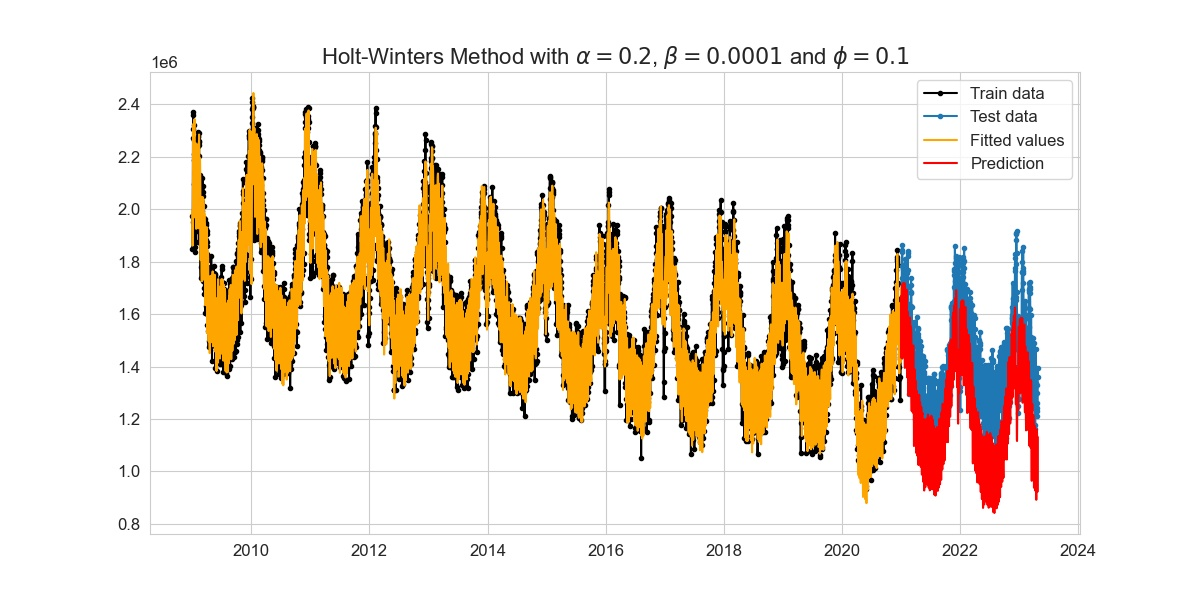
\includegraphics[width = \textwidth]{imagenes/HoltWinters1.jpg}
    \caption{Valores ajustados y predicción del modelo lineal de Holt-Winters}\label{fig:HoltWinters1}
\end{figure}
\begin{figure}[h]
    \centering
    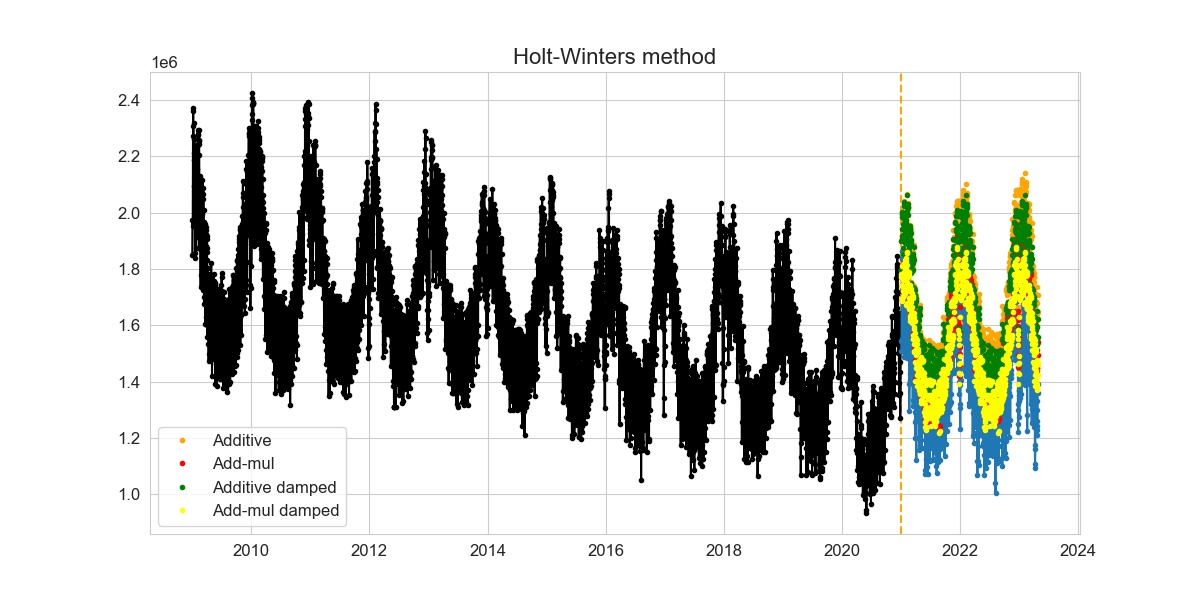
\includegraphics[width = \textwidth]{imagenes/HoltWinters2.jpg}
    \caption{Predicciones de los cuatro modelos del método de Holt-Winters}\label{fig:HoltWinters2}
\end{figure}



\begin{figure}[h]
    \centering
    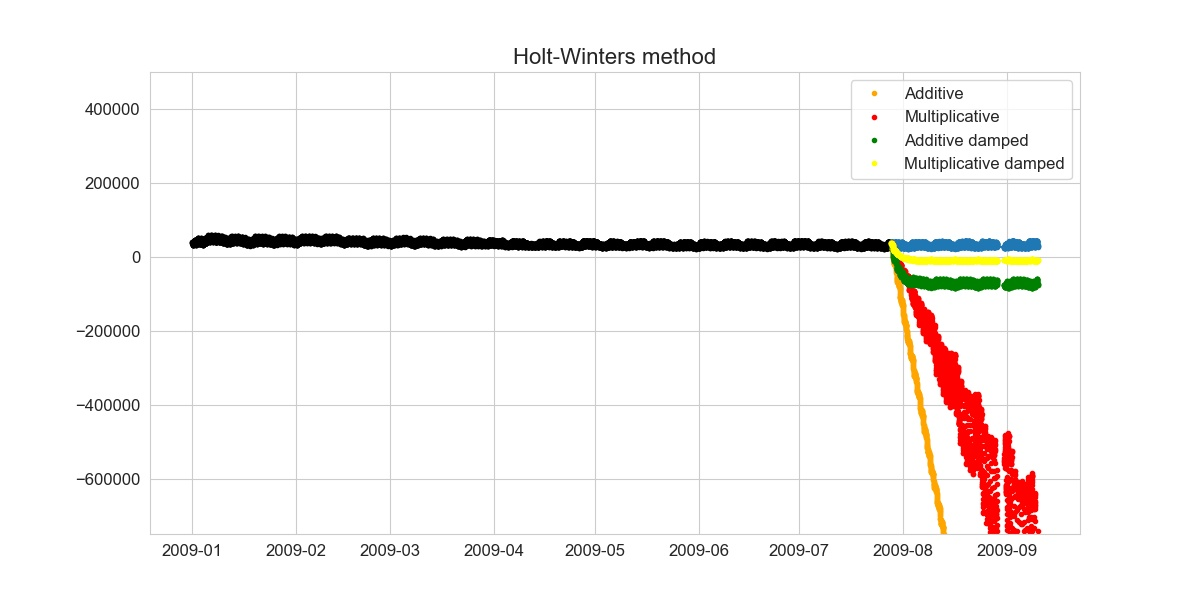
\includegraphics[width = \textwidth]{imagenes/HoltWinters5.jpg}
    \caption{Predicciones del método de Holt-Winters para los datos compeltos}\label{fig:HoltWinters5}
\end{figure}


Por otra parte, se puede ver las limitaciones de este método al aplicarse a los datos completos. El número de observaciones es tan alto que el tiempo de ejecución del algoritmo supera las 10 horas, por tanto se ha aplicado el algoritmo solamente a los primeros meses de los datos. La Figura \ref{fig:HoltWinters5} muestra las predicciones del método y se observa lo nefastas que son. Las predicciones se pueden dividir en dos grupos, las que incluyen el parámetro de amortiguamiento y las que no. Las que no presentan este parámetros se alejan de los valores reales a gran velocidad aumentado el error notablemente. Mientras, los métodos que presentan el parámetro de amortiguamiento son más estables, pero las predicciones de la demanda elétrica para el mes de octubre son negativas, con lo cual no funciona correctamente.

Una limitación de este algoritmo es que no capta correctamente las predicciones a largo plazo, en este caso. Por otra parte, al aumentar el número de observaciones y a su vez el periodo de estacionalidad el tiempo de computación aumenta demasiado, pues tratando con los datos diarios en todos los casos se ejecuta en apenas un segundo.

El algoritmo funciona correctamente modelando los datos diarios, sin embargo aún no se ha encontrado un método de series temporales clásico o de alisado exponencial que permita ajustar a los datos completos. Por ello, en las próximas secciones se presentarán nuevos métodos que conseguirán cumplir dicho objetivo.









\newpage
\section{Prophet}
Prophet es un software de código abierto que fue desarrollado internamente en \emph{Facebook} (ahora conocido como \emph{Meta}) por Sean J. Taylor y Ben Lethan, para afrontar dos de los problemas más comunes en las metodologias de predicción:
\begin{enumerate}
    \item Las herramientas de predicción más automaticas disponibles tienden a ser inflexibles e incapaces de ajustarse a suposiciones adicionales.
    \item La herramientas de predicción más robustas requieres un analisita especializado en la ciencia de datos.
\end{enumerate}

Facebook experimentó demasiada demanda de pronósticos de alta calidad, la cual los analistas no podía proporcionar. En 2017, Facebook lanzó Prophet al público como software de código abierto.

El modelo de Prophet consiste en usar un modelo de series temporales descomponible que tiene en cuenta tres factores importates: la tendencia, la estacionalidad y los días festivos. Estos componentes son combinados en la ecuación
\begin{equation}\label{eq:prophet:descom}
    y(t) = g(t) + s(t) + h(t) + \varepsilon_t .
\end{equation}
El valor de $y$ pronosticado por el modelo en el momento $t$ viene dado por la función $y(t)$. Esta función se descompone en cuatro sumandos:
\begin{itemize}
    \item $g(t)$ se corresponede con la componente de crecimiento o la tendencia general, que modela los cambios no periódicos.
    \item $s(t)$ representa la componente estacional, que es la suma de todos los componentes periódicos.
    \item $h(t)$ representa los efectos de los días festivos, que ocurre en calendarios irregulares durante uno o más días.
    \item $\varepsilon_t$ es el término del error, que engloba todos los demás cambios que no ajustan los demás componentes del modelo.
\end{itemize}

La combianción de estos componentes es todo lo que Prophet requiere para construir las predicciones. Para comprender cómo funciona Prophet es necesario desglosar y estudiar cada uno de los componentes.

\subsection{Modelos de tendencia}
Con el fin de ajustar el componente de tendencias se implementan dos tipos de modelo: un modelo lineal y un modelo logístico. Para pronosticar problemas que no muestran un crecimiento de saturación, una tasa de crecimiento constante por partes proporciona un modelo útil. El modelo lineal se escribe como
\begin{equation} \label{eq:prophet:g_lineal}
    g(t) = (k+\mathbf{a}(t)^T \boldsymbol{\delta})t + (m + \mathbf{a}(t)^T\boldsymbol{\gamma}).
\end{equation}
La variable $k$ es la tasa de crecimiento. Este es un modelo lineal definido a trozos, es decir, la pendiente cambia como una función de $t$, por ello, a la pendiente $k$ se le añade $\mathbf{a}(t)^T\boldsymbol{\delta}$.

Se supone que existen $S$ puntos de cambio en los tiempos $s_j$, $j=1,\dotsc, S$, donde la tasa de crecimiento puede cambiar. Se define el vector de ajustes de tasa $\boldsymbol{\delta}\in \mathbb{R}^S$, donde $\delta_j$ es el cambio en la tasa que ocurre en el tiempo $s_j$. De esta forma, para cualquier tiempo $t$ la tasa es la suma de una tasa base $k$ con todos los ajustes que ocurren hasta este tiempo, es decir, $k + \sum_{j: t>s_j} \delta_j$. Para representarlo de forma más compacta se define el vector $\mathbf{a}(t)\in \{0, 1\}^S$ tal que
\begin{equation*}
    a_j(t) = \left\{ \begin{array}{ll}
        1, & \text{si } t\geq s_j,  \\
        0, & \text{en otro caso.}
    \end{array}\right.
\end{equation*}
De este modo, la tasa para un tiempo dado $t$, es $k + \mathbf{a}(t)^T \boldsymbol{\delta}$. Por último, para que la curva sea continua, es necesario ajustar los segmentos entre cada punto de cambio. Al igual que para la pendiente, el parámetro de compensación es una variable base $m$ añadiendo todos los cambios hasta el tiempo $t$, es decir, $m + \mathbf{a}(t)^T\boldsymbol{\gamma}$, donde $\boldsymbol{\gamma}$ es un vector de ajustes de compensación. En este modelo, con el fin de que la curva sea continua, $\boldsymbol{\gamma}$ se toma de forma que $\gamma_j = - s_j\delta_j$. La Figura \ref{fig:changepoints} muestra un modelo de tendencia lineal con puntos de cambio ajustado a los datos.


\begin{center}
\begin{figure}[h]
    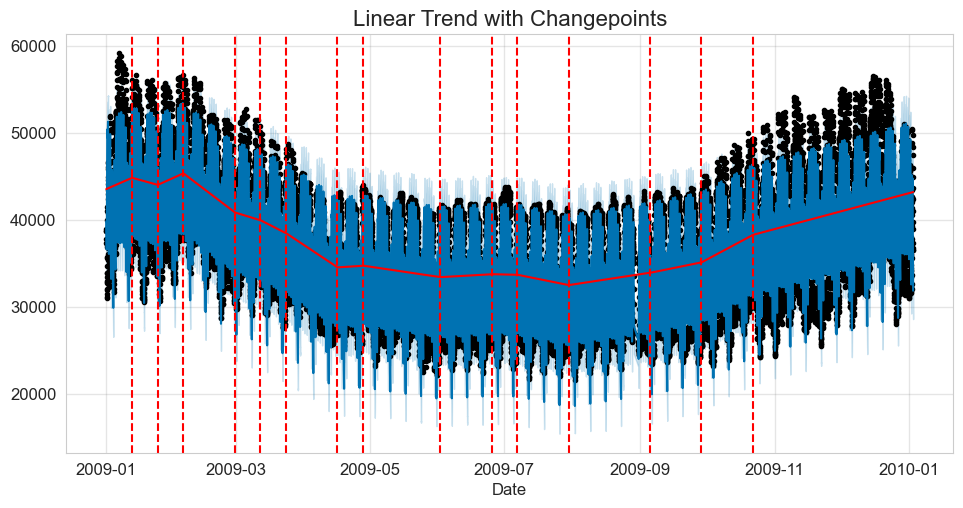
\includegraphics[width = \textwidth]{imagenes/changepoints.png}
    \caption{Modelo de tendencia lineal con puntos de cambio}\label{fig:changepoints}
\end{figure}
\end{center}



Por otro lado, para series temporales que sí presentan un crecimiento de saturación, el factor más importante del proceso es modelar cómo ha crecido la población y cómo se espera que siga creciendo. En este caso se emplea un modelo de crecimiento logístico, dado por la ecuación
\begin{equation}\label{eq:prophet:g_log}
    g(t) = \frac{C}{1 + \exp{(-k(t-m))}},
\end{equation}
donde $C$ es la capacidad de los datos, $k$ la tasa de crecimiento y $m$ un parámetro de compensación. 

El modelo presentado en \eqref{eq:prophet:g_log} tiene sus limitaciones. Primeramente, la capacidad de carga no es siempre constante, por tanto es necesario introducir una función $C(t)$ que represente la capacidad a lo largo del tiempo. Por otra parte, al igual que en el modelo anterior, se plantea la tasa de de crecimiento como $k + \mathbf{a}(t)^T\boldsymbol{\delta}$ y el parámetro de compensación $m + \mathbf{a}(t)^t\boldsymbol{\gamma}$. En este caso, cambian los valores de $\gamma_j$, $j=1,\dotsc,S$, con el fin de conectar correctamente los extremos de los segementos. En este modelo, se tiene que 
\begin{equation}
    \gamma_j = \left(s_j-m-\sum_{l<j}\gamma_l\right)\left(1 - \frac{k+\sum_{l<j}\delta_l}{k+\sum_{l\leq j\delta_l}}\right).
\end{equation}
El modelo de crecimiento logístico por partes es 
\begin{equation}\label{eq:prophet:g_log2}
     g(t) = \frac{C(t)}{1 + \exp{(-(k+\mathbf{a}(t)^T\boldsymbol{\delta})(t-(m+\mathbf{a}(t)^T\boldsymbol{\gamma}))}}.
\end{equation}

\subsection{Estacionalidad}
Los datos de series temporales a menudo exhiben periodicidad, especialmente con datos comerciales, donde a menudo hay ciclos anuales, semanales y diarios. Prophet puede modelar un número ilimitado de dichos componentes periódicos en su término de estacionalidad, $s(t)$, de la ecuación \eqref{eq:prophet:descom}.

Prophet se basa en la series de Fourier para ajustar el componente estacional. Sea $P$ el periodo regular que se espera en la serie temporal, por ejemplo, $P=365.25$ y $P=7$ para efectos que se repiten anual y semanalmente, respectivamente. Los efectos estacionales se aproximan mediante la fórmula

\begin{equation}\label{eq:prophet:s}
    s(t) = \sum_{n=1}^N \left( a_n\cos{\left(\frac{2\pi n t}{P}\right)} + b_n \sin{\left(\frac{2 \pi n t}{P}\right)}\right),
\end{equation}
que consiste en una serie de Fourier estándar. En este caso no se considera el término independiente porque a su vez también se ajusta el componente de tendencia.




Ajustar el modelo \eqref{eq:prophet:s} a los datos requiere estimar un total de $2N$ parámetros, $\boldsymbol{\beta} = [a_1, b_1, \dotsc, a_N, b_N]^T$. Esta estimación se hace a partir de una matriz de estacionalidad con los vectores para cada valor de $t$ de los datos históricos y los datos futuros. Por ejemplo, para estacionalidad semanal y $N=3$, 
\begin{equation*}
    X(t) = \left[ \cos{\left(\frac{2\pi (1)t}{7}\right)} , \sin{\left( \frac{2\pi(1)t}{7}\right)},  \dotsc, \sin{\left( \frac{2\pi(3)t}{7}\right)}  \right].
\end{equation*}
El componente estacional es
\begin{equation}\label{eq:prophet:s2}
    s(t) = X(t) \boldsymbol{\beta}.
\end{equation}

En este modelo generativo se toma $\boldsymbol{\beta} \sim \text{Normal}(0, \sigma^2)$ para imponer un suavizado previo a la estacionalidad. Aumentar $N$ permite ajustar los patrones de los datos que cambian rápidamente, sin embargo este aumento también incrementa el riesgo de sobreajustar el modelo. Para datos con patrones anuales y semanales se ha visto que $N=10$ y $N=3$, respectivamente, funciona correctamente para la mayoria de los problemas.

El algoritmo de Prophet utlizando las series de Fourier es muy práctico a la hora de ajustar los diferentes periodos de estacionalidad. En la Figura \ref{fig:prophet_comp} puede observarse cómo se modelan los componentes anual, semanal y diario de los datos.

\begin{center}
\begin{figure}[h]
    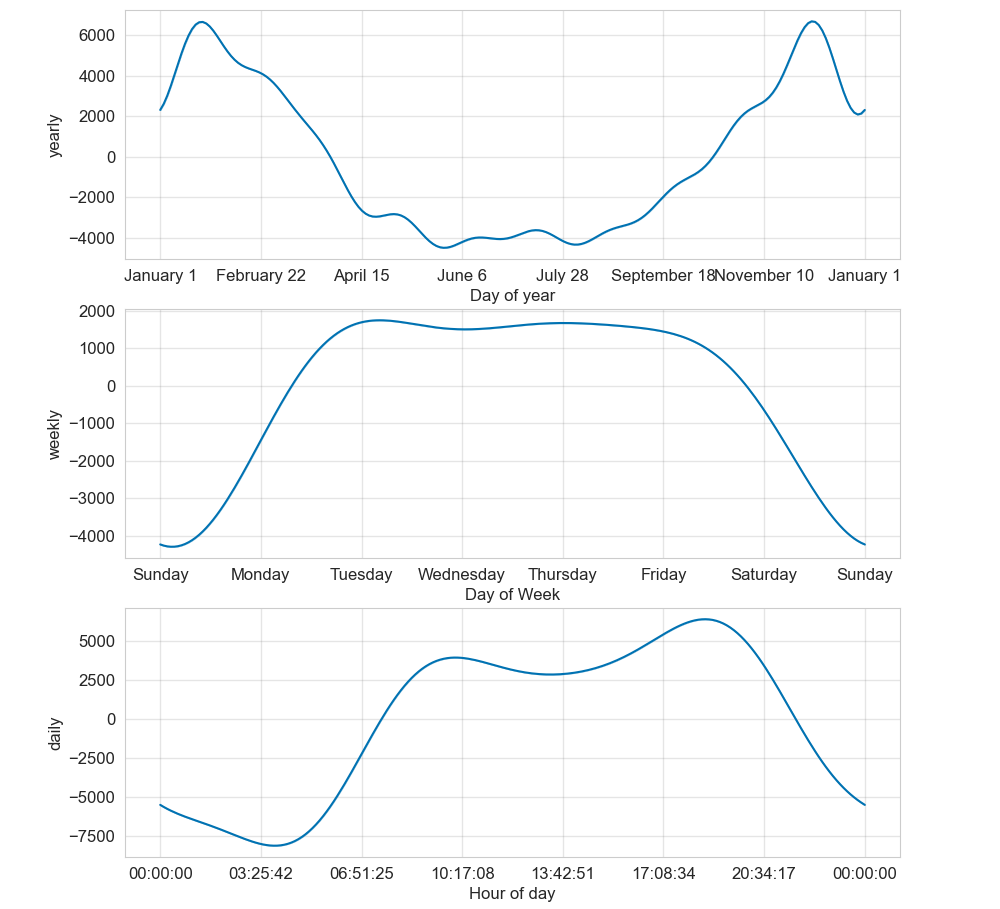
\includegraphics[width = \textwidth]{imagenes/prophet_comp.png}
    \caption{Componentes de estacionalidad del modelo Prophet}\label{fig:prophet_comp}
\end{figure}
\end{center}



\newpage
\subsection{Días festivos y eventos}
Prophet fue diseñado para manejar predicciones de grandes empresas, por lo tanto es importante incluir el efecto que producen los días festivos, que juegan un papel importante en actividades de negocios. Prophet incluye un soporte sólido para incluir los efectos de las vacaciones en sus pronósticos. 

\begin{table}[h] 
\centering
\begin{tabular}{cc} \hline
Holiday & Date \\\hline
New Year's Day & 01-01-2009\\
New Year's Day & 01-01-2010\\
Good Friday & 10-04-2009 \\
Good Friday & 02-04-2010 \\
Good Friday & 22-04-2011 \\ \hline

\end{tabular}
\caption{Días festivos en Reino Unido} \label{tab:festivos}
\end{table}
La incorporación de una lista de días festivos en el modelo se simplifica asumiendo que los efectos de los días festivos son independientes. Para cada día festivo $i$, sea $D_i$ el conjunto de las fechas pasadas y futuras de dicho festivo, la Tabla \ref{tab:festivos} exhibe un ejemplo de cómo se introduce la información de las vacaciones en Python. Se añade una función indicadora que represente si un tiempo $t$ es durante el festivo $i$, y se le asigna a cada vacación el parámetro $\kappa_i$, que es el cambio en la predicción. Se crea una matriz de regresión
\begin{equation*}
    Z(t) = [\mathbf{1}(t\in D_1), \dotsc, \mathbf{1}(t\in D_L)]
\end{equation*}
y se toma 
\begin{equation}\label{eq:prophet:h}
    h(t) = Z(t) \boldsymbol{\kappa}.
    \end{equation}

Al igual que con la estacionalidad, se considera que a priori $\boldsymbol{\kappa} \sim \text{Normal}(0, \nu^2)$. A menudo es importante añadir los efectos de los días festivos en un umbral alrededor de los mismos. Para ello se incluyen parámetros adicionales para los días circundantes a los festivos, tratando estos días como festivos. La Figura \ref{fig:prophet_hday} es un gráfico con los efectos de las vacaciones en el modelo, se observar que para los días festivos la demanda eléctrica tiende a disminuir.




\begin{center}
\begin{figure}[h]
    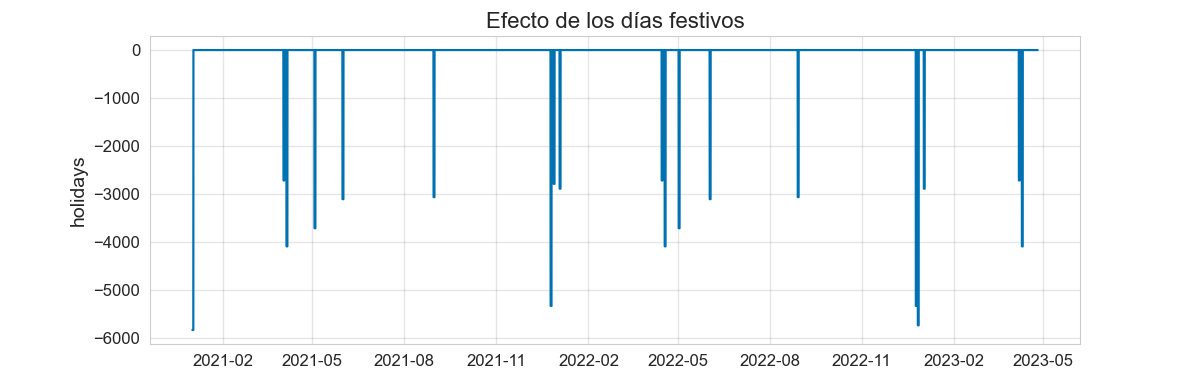
\includegraphics[width = \textwidth]{imagenes/prophet_hday.png}
    \caption{Efecto de los días festivos en los datos}\label{fig:prophet_hday}
\end{figure}
\end{center}

\subsection{Prediciones con Prophet}
En esta sección se va a estudiar la actuación del modelos presentado aplicado a los datos que se dispone. Una vez ajustados todos los componentes de la ecuación \eqref{eq:prophet:descom} el algoritmo se encarga de hacer las predicciones para cualquier valor de $t$.

En las Figuras \ref{fig:prophet_predition} y \ref{fig:prophet_pred2} se muestra las predicciones del modelo. Se observa cómo este modelo sí ha sido capaz de modelar correctamente la componente estacional. Cabe resalta que, hasta el momento, ninguno de los modelos había sido de ajustar el conjunto de datos completo. Y además, se observa en la Figura \ref{fig:prophet_pred2} cómo también ajusta de forma precisa los datos medidos durante las horas del día.

\begin{center}
\begin{figure}[h]
    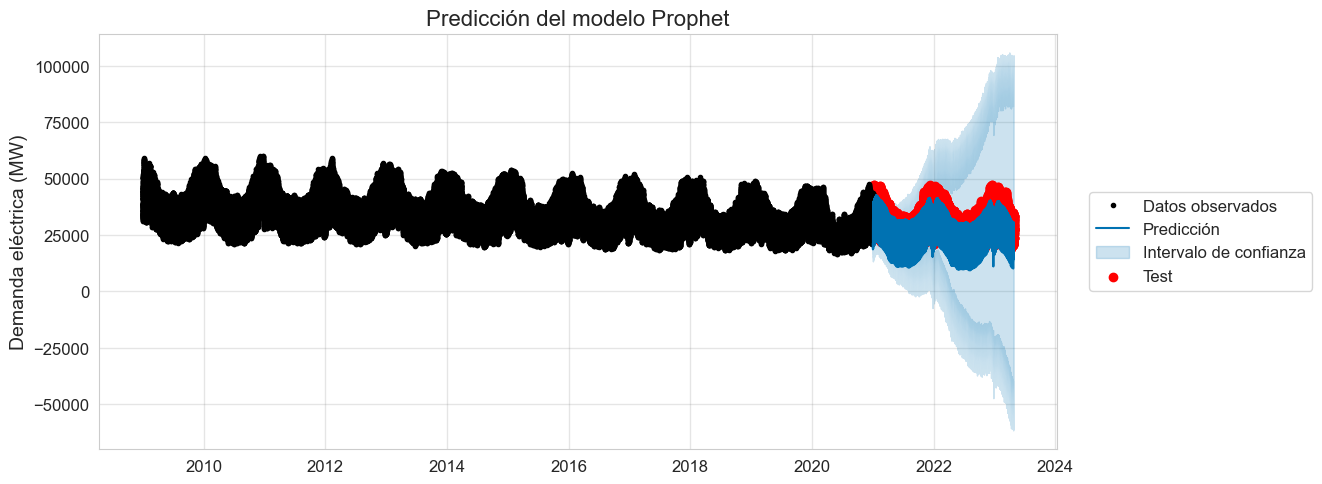
\includegraphics[width = \textwidth]{imagenes/prophet_predition.png}
    \caption{...}\label{fig:prophet_predition}
\end{figure}
\end{center}

El modelo presentado en esta sección tiene implementado los efectos de la vacaciones y gracias a la validación cruzada se ha obtenido los parámetros que minimizan en el error medio absoluto, que en este caso es $11.88\%$. Hasta el momento, es el mejor modelo presentado para modelar los datos y su tiempo de computación es de $18$ minutos y $23$ segundos, siendo unos de los modelos que más tardan pero también el que mejor funciona.

La gran ventaja de este método es que está diseñado para que tanto analistas con grandes conocimientos en la ciencia de datos como personas no tan especializadas puedan ajustar los parámetros para tener predicciones de calidad. En este caso gracias a la validación cruzada se ha encontrado un modelo óptimo en términos de MAPE, sin embargo, con los parámetros prefijados en Python, también se obtienen buenas predicciones, aunque puedan tener menor calidad. 

\newpage
\begin{center}
\begin{figure}[h]
    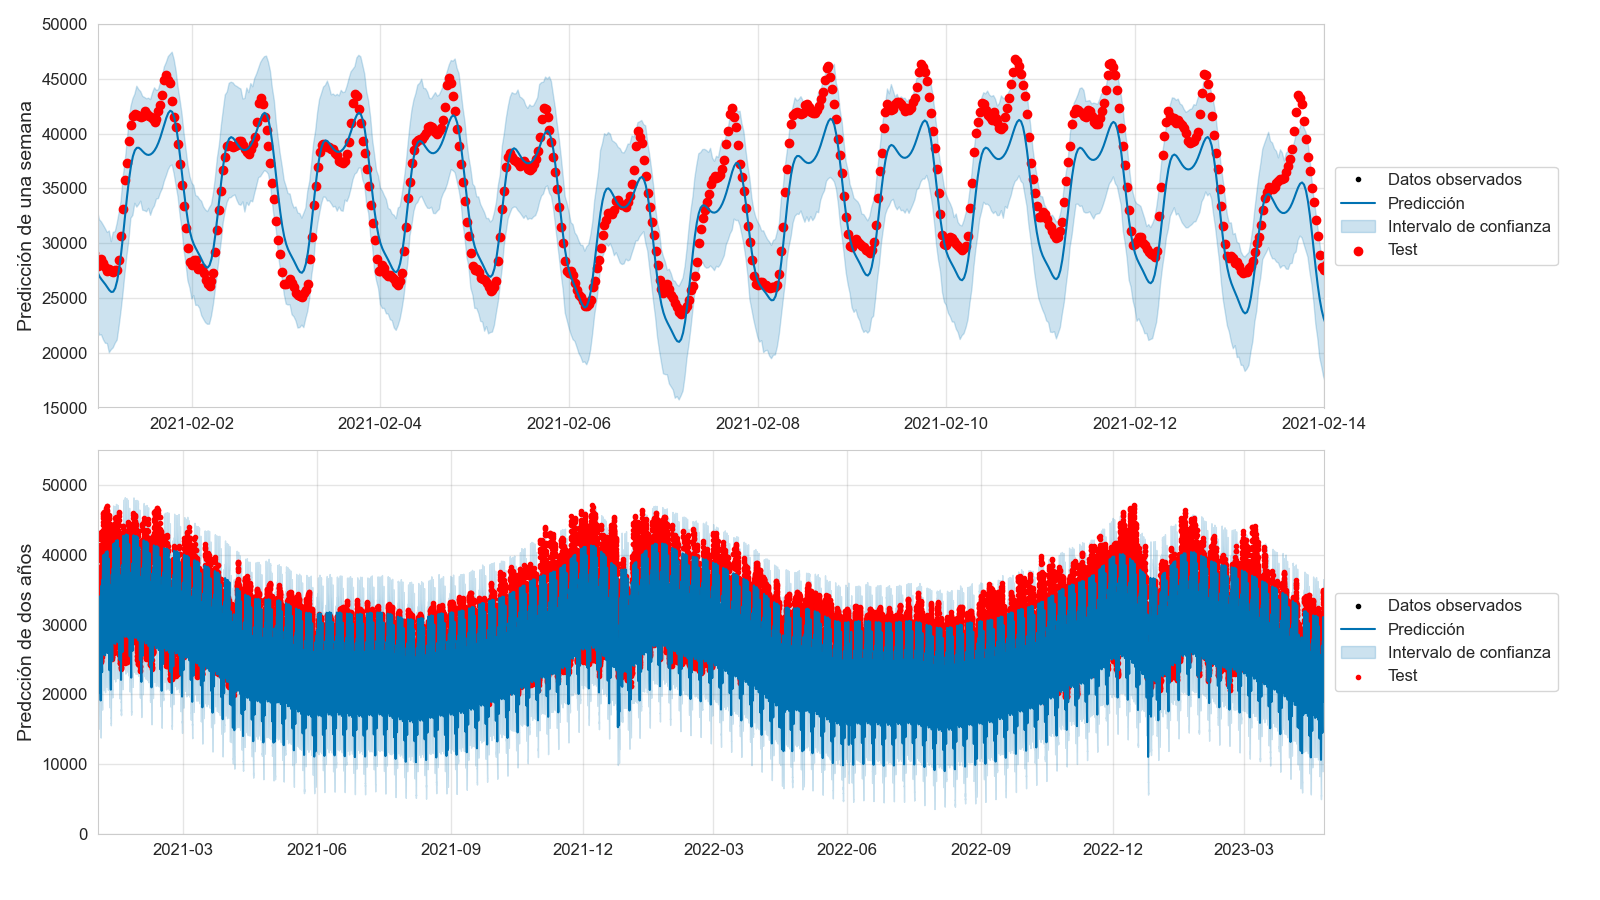
\includegraphics[width = \textwidth]{imagenes/prophet_pred2.png}
    \caption{Predicciones con el modelo Prophet}\label{fig:prophet_pred2}
\end{figure}
\end{center}






\newpage
\section{Modelos autorregresivos con árboles de decisión}


\newpage
\section{Conclusiones}




%-------------------------------------------------------------------------------------------------------

\newpage
\addcontentsline{toc}{section}{Referencias}
\begin{thebibliography}{100}


% ¿cómo citar este?
\bibitem{Prophet1} Taylor SJ, Letham B. 2017. \textit{Forecasting at scale}. PeerJ Preprints 5:e3190v2 https://doi.org/10.7287/peerj.preprints.3190v2

\bibitem{Prophet2} Rafferty, G.,(2023).
\textit{Forecasting Time Series Data with Prophet}. Packt Publishing.  

\bibitem{Prophet3} Korstanje, J., Advanced Forecasting with Python: With State-of-the-Art-Models Including LSTMs, Facebook’s Prophet, and Amazon’s DeepAR in Korstanje, J. (2021) pp.253-271.

\bibitem{TS1} Brockwell, P.J., Davis, R.A.  (1987).
\textit{Time Series: Theory and Methods}. Springer.

\bibitem{TS2} Peña, D.  (2010).
\textit{Análisis de series temporales}. Alianza Editorial.

\bibitem{TS3} Brockwell, P.J., Davis, R.A.  (1996).
\textit{Introduction to Time Series and Forecasting}. Springer.


\bibitem{ES1} Hyndman, R.J., Athanasopoulos, G.  (2014).
\textit{Forecasting: principles and practice}. OTexts.

\bibitem{ES2} Hyndman, R., Koehler, A., Ord, K., Snyder, R.  (2008).
\textit{Forecasting with Exponential Smoothing}. Springer.


% \bibitem{SARIMA01} Wang, S., Li, C. and Lim, A. (2021). \textit{Why Are the ARIMA and SARIMA not Sufficient}.








% \vspace{5cm}
% % Ejemplo de referencia de un libro:
% \bibitem{FA01} Fajardo, M.D., Goberna, M.A., Rodríguez, M.M.L. and Vicente-Pérez, J. (2020).
% \textit{Even Convexity and Optimization: Handling Strict Inequalities}. Springer.

% % Ejemplo de referencia de un capítulo de un libro:
% \bibitem{AR01} Aragón, F.J., Convexity in Nonlinear Optimization in Aragón, F.J., Goberna, M.A., López, M.A. and Rodríguez, M.L. (2019) pp.55-89.

% % Ejemplo de referencia de artículos:
% \bibitem{AL01} Alonso-González, C., Navarro-Pérez, M.A. and Soler-Escrivà, X. (2020). \textit{Flag codes from planar spreads in network coding. Finite Fields and their applications} \textbf{68}, 101745.


% % Ejemplo tesis doctorales:
% \bibitem{CA01} Campoy, R. (2018) Contributions to the Theory and Applications of Projection Algorithms. Tesis doctoral Universidad de Murcia, España.

% % Ejemplo páginas web:
% \bibitem{LE01} LeCun, Y., Cortes, C. and Burges, C.J.C., The MNIST database of handwritten digits. http://yann.lecun.com/exdb/mnist/ (Consultado el 25 de Junio de 2021).


\end{thebibliography}



%-------------------------------------------------------------------------------------------------------
\newpage
\appendix

\section{Detalles del desarrollo del trabajo}


\begin{table}[ht] 
\centering
\begin{tabular}{lc} 
  \hline
 Tarea & Tiempo (horas) \\ 
  \hline
Recopilación de materiales &   ... \\ 
Estudio de bibliografía &   ... \\ 
Elaboración de resultados gráficos/numéricos &  ... \\ 
Redacción de la memoria &  ... \\
 \hline
Total & 150\\
\hline
\end{tabular}
\caption{Tiempo aproximado de dedicación al trabajo} \label{tab{02}}
\end{table}

\begin{table}[ht] 
\centering
\begin{tabular}{llll} 
  \hline
 Asignatura & Páginas & Descripción  \\ 
  \hline
Series Temporales   & ... & - \\ 
Análsis de datos I  & ... & - \\ 
Análsis de datos II & ... & - \\ 
\hline
\end{tabular}
\caption{Asignaturas relacionadas con el trabajo} \label{tab{03}}
\end{table}


\end{document}
